\chapter{Matrix I: Linear Algebraic Equations}\label{eq:matrix-linear}
  
So far our focus has been on numerical methods for calculus. Linear algebra is another major mathematical component in physics, where vectors and matrices are main players. It plays an essential role particularly in quantum mechanics. The numerical methods of linear algebra are also used in other numerical methods in later chapters when we solve multivariate root finding/minimization problems, data fitting, and partial differential equations. It is highly desirable to develop efficient and accurate numerical methods for linear algebra.  Despite that the problem looks very basic, numerical methods to solve it is not trivial. 
In this chapter, various numerical methods for solving linear systems are introduced.

The size of the matrix can be very large in real world applications. Writing a code for large matrices is often complicated.  Fortunately, standard libraries such as LAPACK\cite{lapack} are available for most computer languages and we utilize them.  However, it is dangerous to use such black-box routines without knowing how they work.  In this chapter, basic ideas are introduced using small matrices, mostly 3-by-3.  Once we understand the ideas, we can use the black-box routines with confidence and when they fail we will find alternative methods.

In particular, we are interested in linear algebraic equations.  We often encounter a set of simultaneous equations like 
\begin{subequations} \label{eq:3x3_1}
\begin{eqnarray}
3 x - y + 4 z &=& 2  \label{eq:3x3_1a}\\
2 x -z &=& -1 \label{eq:3x3_1b}\\
3 y + 2z &=&  3\label{eq:3x3_1c}
\end{eqnarray}
\end{subequations}
Writing it in a matrix form, the set of equations are expressed in a single equation  $A \vb{x} = \vb{b}$, where
\begin{equation}\label{eq:3x3_matrix}
A = \begin{bmatrix}
3 & -1 & 4 \\ 2 & 0 & -1 \\ 0 & 3 & 2
\end{bmatrix}
, \qquad
\vb{b}=
\begin{bmatrix}
2 \\ -1 \\ 3
\end{bmatrix}\, .
\end{equation}

To discuss more general cases, we write a system of linear equation in a matrix form
\begin{equation}
\begin{bmatrix}\label{eq:NbyN}
A_{11} & A_{12} & \cdots & A_{1N}\\
A_{21} & A_{22} & \cdots & A_{2N}\\
 &  &  \ddots & & \\
A_{N1} & A_{N2} & \cdots & A_{NN}
\end{bmatrix}
\begin{bmatrix}
 x_1 \\
 x_2 \\
 \vdots\\
 x_N
\end{bmatrix}
=
\begin{bmatrix}
 b_1 \\
 b_2 \\
 \vdots\\
 b_N
\end{bmatrix}
\end{equation}
or simply
\begin{equation}\label{eq:lin_sys}
A \vb{x} = \vb{b}
\end{equation}
where $A$ is a $N$-by-$N$ square matrix, and $\vb{x}$ and $\vb{b}$ are column vectors of length $N$.  Mathematically speaking,
the solution to this equation is as simple as $\vb{x} = A^{-1} \vb{b}$ where $A^{-1}$ the inverse of $A$.  However, finding the inverse matrix is not a trivial task as you know from the linear algebra course. Fortunately, there are smart numerical methods to solve it even without computing the actual inverse matrix. In MATLAB, simply \texttt{x=b$\backslash$A} solves the problem. We can of course use it and it works in most cases.  However, we always need to understand the degree of accuracy and the stability of the numerical method used inside MATLAB. 

When we solve Eq. \eqref{eq:3x3_1} by hand a common method is to eliminate variables one by one (the method of variable elimination).  Numerical methods essentially do the same. 
First, we discuss a trivial case. If the matrix $A$ is either upper or lower triangular, \emph{forward substitution} and \emph{back substitution} solve the problem right away.  For general cases, we introduce numerical methods known as \emph{Gaussian elimination} and $LU$ decomposition, which transform general matrix problems to triangular matrix problems.

\noindent
\section{Triangular Matrices}

We first discuss a special kind of matrices: lower triangular matrix
\begin{equation}\label{eq:matrix_L}
L = \begin{bmatrix} L_{11} & 0 & 0 & \cdots & 0 \\ L_{21} & L_{22} & 0 & \cdots & 0\\ L_{31} & L_{32} & L_{33} & \cdots & 0 \\
 \vdots & \vdots & \vdots & \ddots  & 0 \\
L_{N1} & L_{N2}& L_{N3}& \cdots &L_{NN}
 \end{bmatrix},
\end{equation}
and upper triangular matrix
\begin{equation}\label{eq:matrix_U}
U = \begin{bmatrix} U_{11} & U_{12} & U_{13} & \cdots & U_{1N} \\0 & U_{22} & U_{23}  & \cdots & U_{2N} \\ 0 & 0 & U_{33}  & \cdots & U_{3N} \\0 & \vdots & \vdots & \ddots & \vdots \\ 0& 0& 0& 0& U_{NN} \end{bmatrix}.
\end{equation}
The triangular matrices have several nice properties such as
\begin{center}
\begin{minipage}{6in}
\begin{itemize}[labelwidth=0.5cm,labelindent=0cm,leftmargin=*,align=left]
\item The product of two same type of triangular matrices is again the same type of a triangular matrix.
\item The inverse of a triangular matrix is the same type of triangular matrix as the original one.
\item The determinant of a triangular matrix is just a product of all diagonal elements.
\end{itemize}
\end{minipage}
\end{center}

\begin{example}
To familiarize ourselves with triangular matrices, we verify the above properties numerically.
Since we have not learned how to evaluate matrix inverse and determinant,  we use MATLAB built-in functions, \texttt{inv()} and \texttt{det()}. Numerical methods to compute them will be discussed in this chapter.
Let us verify the three properties using the following lower triangular matrix,
\begin{equation}
A = \begin{bmatrix}
2 & 0 & 0 \\ -1 & 1& 0\\ 3 & 2 & -1 
\end{bmatrix}, \qquad
B = \begin{bmatrix}
1 & 0 & 0 \\ 2 & 4& 0\\ -1 & -2 & 3 
\end{bmatrix}.
\end{equation}
Program \ref{prog:triangular_matrix} computes the product of $A$ and $B$, inverse and determinant of $A$.  Here is the outputs.
\begin{mybox}

\small
\begin{verbatim}
Mutilication: A*B
  2   0   0
  1   4   0
  8  10  -3

Inverse of A
     5.0000e-01     -5.5511e-17      5.5511e-17
     5.0000e-01      1.0000e+00      0.0000e+00
     2.5000e+00      2.0000e+00     -1.0000e+00

Products of the diagonal elements = -2
Determinant by MATLAB = -2.000000e+00
\end{verbatim}
\normalsize
\end{mybox}
The product is again a lower triangular matrix.  The inverse is not exactly a lower triangular matrix since the upper triangle elements are not exactly zero. They are numerical errors caused mostly by round-off error and  practically small enough to be ignored.  Finally, the product of the diagonal elements matches to the determinant obtained by the built-in function.
\end{example}

\noindent
\subsection{Forward/Back Substitutions}
First, we will solve a simple linear equation 
\begin{equation}\label{eq:Lx=b}
L \vb{x} = \vb{b}
\end{equation}
where the matrix $L$ is lower triangular.   For simplicity, we consider 3-by-3 matrices but the method will work for any size of matrices.

Writing Eq. \eqref{eq:Lx=b} explicitly, the corresponding equations of the system is
\begin{subequations}
\begin{eqnarray}
L_{11} x_1 &=& b_1 \\
L_{21} x_1 + L_{22} x_2 &=& b_2 \\
L_{31} x_1 + L_{32} x_2 + L_{33} x_3 &=& b_3
\end{eqnarray}
\end{subequations}
It is trivial to solve this equation.  From the first equation, $x_1 = b_1/L_{11}$. Solving the second equation for $x_2$, we obtain
$x_2 = (b_2 -L_{21} x_1)/L_{22} = (b_2 - b_1 L_{21}/L_{11}) / L_{22}$. $x_3$ can be obtained in the same way.  For general cases, the solution is given by
\begin{equation}\label{eq:fwd_sb}
x_i=\frac{1}{L_{ii}} \left( b_i - \displaystyle\sum_{j=1}^{i-1} L_{ij} x_j\right )
\end{equation}
In order to find $x_i$, we must know $x_1, x_2, \cdots, x_{i-1}$.  In other words, you must evaluate this equation in the forward order from $i=1$ to $N$. That is why this method is called \emph{forward substitution}.  

Similarly for the upper triangular matrix, $U \vb{x} = \vb{b}$ can be solved easily by back substitution
\begin{equation}\label{eq:bwd_sb}
x_i=\frac{1}{U_{ii}} \left ( b_i - \displaystyle\sum_{j=1+1}^{N} U_{ij} x_j \right )
\end{equation}
which must be evaluated backward from $i=N$ to $i=1$ and thus this method is known as \emph{back substituion}.

\bigskip
\begin{example}
We solve the following equation.
\begin{subequations}
\begin{eqnarray} \label{eq:bs}
3 x - y + 4 z &=& -1\label{eq:bs1} \\
2 y -z &=& -2\label{eq:bs2}\\
2z &=& 4 \label{eq:bs3}
\end{eqnarray}
\end{subequations}
First, we write it in  matrix form
\begin{equation}
\begin{bmatrix}
3 & -1 & 4 \\ 0 & 2 & -1 \\ 0 & 0& 2
\end{bmatrix}
\begin{bmatrix}
x \\ y \\ z
\end{bmatrix}
=
\begin{bmatrix}
-1 \\ -2 \\ 4
\end{bmatrix}.
\end{equation}
Since the matrix is upper triangular, we use the back substitution method. Program \ref{prog:triangular_matrix2} carries out back substitution and the solution is

\medskip
\begin{mybox}
   
   \medskip
   \begin{verbatim}
      x=-3.0, y=0.0, z=2.0
   \end{verbatim}
\end{mybox}
\end{example}

\noindent
\section{Gaussian Elimination}

Solving linear equations of triangular matrix is almost trivial. Is there a similar formula for general matrix problems?  The answer is NO.  The problem is much harder.  However, almost any general matrix problem can be transformed to an equivalent triangular matrix problem as long as $A$ is not singular.  Since a non-trivial problem becomes a trivial problem, the transformation procedure must be non-trivial (due to the law of the conservation of difficulty).  The procedure is actually the same as what we do when we solve the equation manually by hand. That is the method of variable elimination which is commonly known as \emph{Gaussian elimination}.

\subsection{Elmination Procedures}

First, let us solve  \eqref{eq:3x3_1} by hand. Diagram \eqref{eq:gaussian_elimination} shows it.  First, we eliminate $x$ in the second equation  using the first equation.   From the first equation $x=\frac{1}{3}(y -4z +2)$.  Substituting it to the second equation, $x$ in the second equation is eliminated.  Next, we do the same for the third equation. This time, we will eliminate $y$.  The third equation contains only $z$ and thus we solve the problem. Notice that the final expression is upper triangle. 
The second equation can be simplified by multiplying $3$ to both sides.  However, that will change the properties of the matrix, namely the determinant.  So, we keep the rather messy expression.

\small
\begin{subequations}\label{eq:gaussian_elimination}
\begin{align}
3 x - y + 4 z &= 2  & 3 x - y + 4 z &= 2 & 3 x - y + 4 z &= 2 \\
2 x -z &= -1  &\xrightarrow[\text{elimination}]{\text{1 st}} \quad  \frac{2}{3} y - \frac{11}{3} z &= -\frac{7}{3} & \xrightarrow[\text{elimination}]{\text{2 nd}} \quad
\frac{2}{3} y - \frac{11}{3} z &= -\frac{7}{3} \\
3 y + 2z &=  3 & 3 y + 2z &=  3 & \frac{37}{2} z &=  \frac{27}{2}
\end{align}
\end{subequations}
\normalsize


Now we write this procedure in a matrix form,
\begin{equation}
A \vb{x}=\vb{b} \quad \Rightarrow  \quad M^{(1)} A \vb{x}= M^{(1)} \vb{b} \quad \Rightarrow \quad M^{(2)} M^{(1)} A \vb{x}= M^{(2)} M^{(1)} \vb{b}.
\end{equation}
where the transformation matrix $M^{(i)}$ applies the $i$-th step of the forward Gaussian elimination. For the above example, the transformation matrices are
\begin{equation}
M^{(1)} = \begin{bmatrix}1 & 0 & 0\\ -2/3 & 1 & 0 \\ 0 & 0 & 1 \end{bmatrix}, \qquad M^{(2)} = \begin{bmatrix}1 & 0 & 0\\ 0 & 1 & 0 \\ 0 & -9/2 & 1 \end{bmatrix}.
\end{equation}
Notice that these matrices are lower triangular matrices and only one element differs from the identity matrix.

In general,  the product of $N-1$ transformation matrices transforms a general linear equation to an upper triangular equation.
\begin{equation}\label{eq:gaussian-elimination-matrix}
M^{(N-1)} M^{(N-2)} \cdots M^{(2)} M^{(1)} A \vb{x}=M^{(N-1)} M^{(N-2)} \cdots M^{(2)} M^{(1)}\vb{b} \longrightarrow U\vb{x}=\vb{b}' 
\end{equation}
Note that the transformation matrix is applied to the both sides of the equation.  In other words, we are modifying $\vb{b}$ as well as $A$, which is a weak point of the Gaussian elimination method which we will discuss later.
Algorithm \ref{algo:gaussian_elimination} shows the summary of the Gaussian forward elimination procedure.

\begin{myalgobox}
   \Algorithm{Gaussian forward elimination}\label{algo:gaussian_elimination}
   
   \medskip
   \begin{enumerate}
      \item  Consider a recursive equation $A^{(n+1)} = M^{(n)} A^{(n)}$ and $\vb{b}^{(n+1)} = M^{(n)} \vb{b}^{(n)}$, starting with the original equation $A^{(1)} \vb{x} = \vb{b}^{(1)}$ where $A^{(1)}$ is a $N$-by-$N$ matrix.

      \item  $M^{(n)}$ is the same as the identity matrix except for the $n$-th column,\\  $M^{(n)}_{kn}=-A^{(n)}_{kn}/A^{(n)}_{nn}$ where $k=n+1, \cdots, N$.
      
      \item  Apply the transformation to both $A^{(n)}$ and $\vb{b}^{(n)}$. Note that the transformation affect only the rows from $n+1$ to $N$ of $A^{(n)}$ and $\vb{b}^{(n)}$.
      
      \item  Increment $n$ and repeat from step 2 until $n=N$.
   \end{enumerate}
\end{myalgobox}

Although the method is simple and works fine for many cases, it fails when the matrix is close to singular. There are better methods. We introduced the Gaussian elimination method for a pedagogical purpose since similar ideas are used in other methods.  More practical methods will be discussed later.

\bigskip
\begin{example}\label{ex:gaussian_elimination}

We solve Eq. \eqref{eq:3x3_1} using the Gaussian elimination followed by the back substitution.  Program \ref{prog:gaussian_elimination} implements Algorithm \ref{algo:gaussian_elimination}.  The following output shows the linear equation after Gaussian elimination is applied.  The matrix $A$ is transformed to a upper triangular form and $b$ is also transformed accordingly.   Then, the solution $x$ is obtained from the transformed equation by the back substitution, which is in agreement with the exact solution $x=-\displaystyle\frac{5}{37}$, $y=\displaystyle\frac{19}{37}$, $z=\displaystyle\frac{27}{37} $.


\begin{mybox}
\small
\begin{verbatim}
A=
 3.00000  -1.00000   4.00000
 0.00000   0.66667  -3.66667
 0.00000   0.00000  18.50000

b=
 2.00000
-2.33333
13.50000

x=
-0.13514
 0.51351
 0.72973
\end{verbatim}
\normalsize
\end{mybox}
\end{example}

\noindent
\subsection{Pivoting}

The Gaussian elimination method suffers from round-off errors, sometimes severely. To see the source of the error, apply the Gaussian elimination to the following problem:

\small
\begin{subequations}
\begin{align*}
\epsilon x + y + z &= 1 &  \epsilon x + y + z &= 1 & \epsilon x + y + z &= 1 \\
x + y &= 2 & \xrightarrow[\text{elimination}]{\text{1st}} \quad \left (1-\frac{1}{\epsilon}\right )y - \frac{1}{\epsilon} z &= 2 - \frac{1}{\epsilon}
&  \xrightarrow[\text{round-off}]{\epsilon \rightarrow 0} \quad -\frac{1}{\epsilon}y - \frac{1}{\epsilon} z &= - \frac{1}{\epsilon}\\
x + z &= 3 & -\frac{1}{\epsilon} y + \left ( 1-\frac{1}{\epsilon} \right ) z &= 3 - \frac{1}{\epsilon}  &
-\frac{1}{\epsilon} y - \frac{1}{\epsilon} z &=  - \frac{1}{\epsilon}
\end{align*}
\end{subequations}
\normalsize
where $\epsilon \ll 1$.  Using the first equation, we eliminate $x$ from the second and third equations. As $\epsilon \rightarrow 0$, $\displaystyle\frac{1}{\epsilon}$ becomes so large that computers cannot distinguish $1 - \displaystyle\frac{1}{\epsilon}$ and $- \displaystyle\frac{1}{\epsilon}$ due to round-off. Now the second and third equations are identical and thus there is no unique solution.  On the other hand, when $\epsilon=0$, the solution does exist and it is $x=2, y=0, z=1$.  This example demonstrates the failure of the Gaussian elimination.  

Fortunately, there is a way to avoid such errors.  We did not have to use the first equation to eliminate $x$. Instead, use the second equation to eliminate $x$ in two other equations.  After swapping the first and second rows, we apply the regular Gaussian elimination.

\small
\begin{align*}
x + y &= 2 &  x + y &= 2  & x + y &= 2  \\
\epsilon x + y + z &= 1 & \xrightarrow[\text{elimination}]{\text{1st}} \quad (1-\epsilon) y + z &= 1 - 2 \epsilon & \xrightarrow[\text{elimination}]{\text{2nd}} \quad (1-\epsilon) y + z &= 1 - 2 \epsilon \\
x + z &= 3 & -y + z &= 1 & \frac{2-\epsilon}{1-\epsilon} z &= \frac{2-3\epsilon}{1-\epsilon}
\end{align*}
\normalsize

\begin{center}
$\xrightarrow[\text{round-off}]{\epsilon \rightarrow 0}$
\begin{minipage}[m]{0.4\textwidth}
\small
\begin{subequations}
\begin{eqnarray*}
x + y &=& 2 \\
y + z &=& 1 \\
2 z &=& 2
\end{eqnarray*}
\end{subequations}
\end{minipage}
\end{center}


\medskip
\noindent
After the first step, we don't see any extreme value.
Now, we eliminate $y$ using the second equation.   If the new coefficient to $y$ happened to be very small, we need to swap the second and third equations to avoid the round-off error.   Since the coefficient to $y$ is not small in this example, we don't need to worry about it.  We now go ahead and eliminate $y$. The final expression takes an upper triangular form. When $\epsilon=0$, we obtain the correct solution by the back substitution.

This algorithm of avoiding the round-off errors by rearranging the equations is known as pivoting.  The above example swapped two rows.  This is known as partial pivoting.  In some cases, interchanging both rows and columns may be needed to achieve a desired accuracy. This is known as complete pivoting. We must recall that when the matrix $A$ is singular (the determinant of $A$ is zero) Eq. (\ref{eq:lin_sys}) does not have a unique solution.  When $A$ is near singular (the determinant is close to zero) the Gaussian elimination in general fails even with pivoting. Then, we must resort to other method such as singular value decomposition (SVD)\cite{matrix_comp}.

Algorithm \ref{algo:pivot} summarizes the so-called scaled partial pivoting method.  The basic idea is that when we eliminate a variable $x_n$, we look for the row which has the largest coefficient to $x_n$ (the pivot element).  However, the absolute magnitude of the coefficients does not have significant meaning since each row can be scaled by multiplying a constant without changing the solution.  So, we normalize each row by the largest coefficient in the row. 

\begin{myalgobox}
\Algorithm{Scaled Partial Pivoting}\label{algo:pivot}

\medskip
\begin{itemize}
\item[1.] Find a scale factor for each row.  $S_i = \max_j (|A_{ij}|)$.
\item[2.] Staring with $n=1$, repeat the following procedure up to $n=N-1$.
\item[3.] Assume that $n-1$ variables are already eliminated and the first $n-1$ rows are already upper triangular.  The remaining submatrix  is still not triangular. (See Fig. \ref{fig:fwd_elimination}.)  Now, we eliminate $x_n$. 
\item[4.] Find a row $j \ge n$ such that $|A_{jn}|/S_j \ge |A_{kn}|/S_k,\quad (\forall k \ge n)$.  This is the pivot row.
\item[5.] Move $j$-th row to the top of the submatrix. (Pivoting)
\item[6.] Apply the forward elimination to the row below the pivot row. After that, we have a new $A$ and $b$.
\item[7.] If $n=N-1$, the elimination is completed.  Otherwise, increment $n$ and go to step 3.
\end{itemize}
\end{myalgobox}


\begin{figure}
\centering
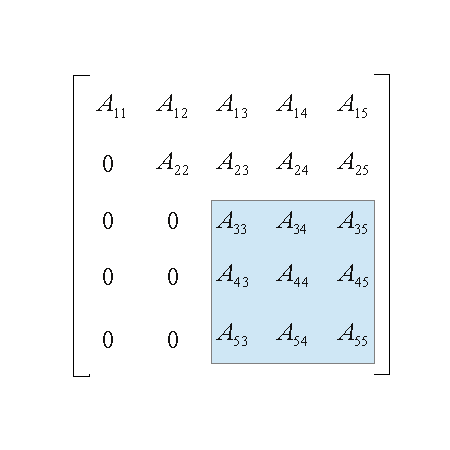
\includegraphics[width=2in]{08.matrix1/gaussian_fwd_elimination.pdf}
\caption{After two steps of forward elimination, 3-by-3 submatrix remains non-triangular. To find the next pivot,
find the maximum of $A_{33}/S_3$, $A_{43}/S_4$, and $A_{53}/S_5$. The row carrying the maximum goes to the top of the submatrix.}
\label{fig:fwd_elimination}
\end{figure}

\bigskip
\begin{example}\label{ex:gaussian_elimination_pivot}
We solve Eq. \eqref{eq:3x3_1} again but using partial pivoting this time. Program \ref{prog:gaussian_elimination_pivot} will do it.
The permutation matrix $P$ indicates which rows are swapped.
The results show that the first elimination swapped the first and second rows.  Then, the second elimination interchanged the second and third rows.  The final triangular form of $A$ is totally different from the one obtained without pivoting (see example \ref{ex:gaussian_elimination}).  However, the final solution $\vb{x}$  agrees with the previous example.  Note that the final triangular matrix in Example \ref{ex:gaussian_elimination} contains a large element 18.5.  However, the pivoting avoided the appearance of such a large element.
\begin{center}
\begin{minipage}{2.5in}
\small
\begin{Verbatim}[frame=single]
A=
 2.00000   0.00000  -1.00000
 0.00000   3.00000   2.00000
 0.00000   0.00000   6.16667

b=
-1.00000
 3.00000
 4.50000

P=
0  1  0
1  0  1
0  1  0

x=
-0.13514
 0.51351
 0.72973
\end{Verbatim}
\normalsize
\end{minipage}
\end{center}

\end{example}

\noindent
\subsection{Determinant}

The determinant of a triangular matrix is simple.  Just the product of the all diagonal is the determinant. For example, an upper triangular matrix $U$ has the determinant:
\begin{equation}
|U| = \prod_i^{N} U_{ii}.
\end{equation}
Now, we show that the Gaussian elimination preserves the determinant. Using the transform matrices defined in Eq. \eqref{eq:gaussian-elimination-matrix}, the final upper triangular form $U$ is given by
\begin{equation}\label{eq:total_M}
U = M^{(N-1)} M^{(N-2)} \cdots M^{(2)} M^{(1)} A
\end{equation}
and its determinant
\begin{equation}
|U| = |M^{(N-1)} M^{(N-2)} \cdots M^{(2)} M^{(1)} A| = |M^{(N-1)}| |M^{(N-2)}| \cdots |M^{(2)}| |M^{(1)}| |A|
\end{equation}
Noting that $M^{(n)}$ is a lower triangular matrix with a unit diagonal, its determinant is 1.  Hence, $|U|=|A|$.
When pivoting is used, 
\begin{equation}
|U| =  |M^{(N-1)}| |P^{(N-1)}| |M^{(N-2)}| |P^{(N-2)}| \cdots |M^{(1)}| |P^{(1)}| |A| = (-1)^p |A|
\end{equation}
where $p$ is the number of pivoting. The proof is simple. If two rows are swapped $|P^{(n)}|=-1$ and otherwise it is $|P^{(n)}|=+1$.

\begin{example}
We calculate the determinant of the matrix in Eq. \eqref{eq:3x3_matrix}.
By using the rule of Sarrus, its determinant is 37.  Now, look at Eq. \eqref{eq:gaussian_elimination}. The corresponding matrix take a upper triangular form:
\begin{equation}
\begin{bmatrix} 3 & -1 & 4 \\ 0 & 2/3 & -11/3 \\ 0 & 0 & 37/2 \end{bmatrix}
\end{equation}
The product of the all diagonal elements is $3 \times 2/3 \times 37/2 = 37$ which is the determinant. 
\end{example}

\noindent
\subsection{Matrix Inversion}

The Gaussian elimination cleverly solves equation $A \vb{x} = \vb{b}$ without deriving $A^{-1}$. However, since we are able to calculate $\vb{x}$, there must be a way to find $A^{-1}$.
Indeed, the Gaussian elimination method can be used to get the inverse. Consider $N$ sets of the linear equations with unit vectors as $\vb{b}$.
\begin{equation}
\begin{bmatrix}  & & \\  & A_{ij} & \\  & &  \end{bmatrix}
\begin{bmatrix} x_{11} \\ x_{21} \\ x_{31} \end{bmatrix}
= \begin{bmatrix} 1\\ 0 \\ 0 \end{bmatrix}, \quad
\begin{bmatrix}  & & \\  & A_{ij} & \\  & &  \end{bmatrix}
\begin{bmatrix} x_{12} \\ x_{22} \\ x_{32} \end{bmatrix}
= \begin{bmatrix} 0 \\ 1\\ 0 \end{bmatrix}, \quad
\begin{bmatrix}  & & \\  & A_{ij} & \\  & &  \end{bmatrix}
\begin{bmatrix} x_{13} \\ x_{23} \\ x_{33} \end{bmatrix}
= \begin{bmatrix} 0 \\ 0 \\ 1 \end{bmatrix}, \quad
\end{equation}
Each equation can be solved by the Gaussian elimination.  Therefore, we have $x_{ij}$.  Now, we can write the set of equations in a single matrix equation
\begin{equation}\label{eq:gauss-jordin}
\begin{bmatrix}  & & \\  & A_{ij} & \\  & &  \end{bmatrix} 
\begin{bmatrix}  & & \\  & x_{ij} & \\  & &  \end{bmatrix} 
=
\begin{bmatrix}  & & \\  & I_{ij} & \\  & &  \end{bmatrix} 
\end{equation}
where $I_{ij}$ is an identity matrix.  Therefore, the matrix $x$ is the inverse of $A$.  By performing Gaussian elimination $N$ times, we can find the inverse of a matrix.  This method is known as Gauss-Jordan elimination. Since this is based on the Gaussian elimination method, it may suffer from round-off error. Other methods are usually used in practical applications. However, it is very useful to know the basic idea of Gauss-Jordan method in order to develop other methods.

\bigskip
\begin{example}

We calculate the inverse of matrix $A$ in Eq \eqref{eq:3x3_matrix}) using the Gaussian elimination.
It is trivial to modify the code in Example \ref{ex:gaussian_elimination_pivot}.  Program \ref{prog:matrix_inverse} calculates the inverse and check the answer by calculating $A\, A^{-1}$. The output show that we recover the identity matrix and thus the inverse is accurate. 

\begin{mybox}

\small
\begin{verbatim}
Invers of A=
 0.08108  -0.10811   0.16216
 0.37838   0.16216  -0.24324
 0.02703   0.29730   0.05405

A A^(-1)=
 1.00000   0.00000   0.00000
 0.00000   1.00000  -0.00000
-0.00000   0.00000   1.00000
\end{verbatim}
\normalsize
\end{mybox}
\end{example}


\noindent
\section{$LU$ Decomposition}

While it is simple, the Gaussian elimination has various weakness.  We reduced the chance of round-off error by pivoting.  Another issue arises when we want to solve the equation many times with the same $A$ but different $\vb{b}$.  We have to carry out the elimination for every different $\vb{b}$ even with the same $A$.  For a large system, that is annoying.  Fortunately, there are better ways.  $LU$ decomposition\cite{matrix_comp} is one of them.

\subsection{Decomposition Algorithm}
Looking at Eq. \eqref{eq:total_M} again. $U=M A$ where $M=M^{(N-1)} M^{(N-2)} \cdots M^{(1)}$.  Recall that $U$ is upper triangular and each $M^{(n)}$ is lower triangular.  Now, using the properties of triangular matrices:  (1) the product of triangular matrices is again the same kind of triangular matrix. (2) the inverse of a triangular matrix is again the same kind of triangular matrix.  Hence, $M$ is lower triangular and so is $M^{-1}$. Let $L=M^{-1}$, we conclude that
\begin{equation}
A = L U
\end{equation}
which is called $LU$ decomposition or $LU$ factorization of $A$.  If pivoting is used, the rows are shuffled.  Therefore,
\begin{equation}
P A = L U
\end{equation}
where $P$ is a permutation matrix. Using the property of permutation, namely $P^{-1} = P$, we obtain a more popular expression
\begin{equation}
A = P L U
\end{equation}
This is just another way to express the Gaussian elimination.  However, this decomposition does not depend of the right hand side $\vb{b}$.  You need to carry out the decomposition only once for $A$.  This saves computer time significantly if $Ax=b$  has to be solved many times with different $\vb{b}$.

MATLAB has a built-in function \texttt{lu()} to compute $LU$ decomposition (See Example \ref{ex:LU}.) For other languages, LAPACK includes LU decomposition routines. Actually MATLAB internally calls LAPACK routines.  Be reminded that any numerical algorithm has weakness.  A blind use of ``canned'' routines is dangerous. We should  carefully check possible pitfalls whenever we use canned routines.

\subsection{Linear equations}
Now, we solve $A \vb{x}=\vb{b}$ using the $LU$ decomposition. The equation is now $P L U \vb{x} = \vb{b}$ or equivalently $LU \vb{x} = P \vb{b}$, which can be divided to two equations, $L \vb{y} = P \vb{b}$ and $U \vb{x} = \vb{y}$ where $\vb{y}$ is an auxiliary vector.  The former equation can be solved for $\vb{y}$ easily by forward substitution.  Then, solve the latter for $\vb{x}$ with back substitution.  Once $L$ and $U$ are computed for $A$, we can use them for different $\vb{b}$ with the same $L$ and $U$. That is a huge advantage. 

\bigskip
\begin{example}\label{ex:LU}

Here is another attempt to solve Eq. (\ref{eq:3x3_1}).  This time we use LU decomposition (built-in function in MATLAB). 
The permutation matrix indicated that the second and third rows are swapped during the decomposition procedure. The product $PLU$ recovers the original $A$. The results agree perfectly with the analytic answers.
\end{example}

\begin{mybox}

\small
\begin{verbatim}
L (Lower Triangular Matrix)
 1.00000   0.00000   0.00000
 0.00000   1.00000   0.00000
 0.66667   0.22222   1.00000

U (Upper Triangular Matrix)
 3.00000  -1.00000   4.00000
 0.00000   3.00000   2.00000
 0.00000   0.00000  -4.11111

P (Permutation Matrix)
1  0  0
0  0  1
0  1  0

P*L*U
 3.00000  -1.00000   4.00000
 2.00000   0.00000  -1.00000
 0.00000   3.00000   2.00000

x=-0.13514,  y=0.51351, z=0.72973
\end{verbatim}
\normalsize
\end{mybox}

\noindent
\subsection{Matrix Inverse}

It is straight forward to find the inverse of a matrix using $LU$ decomposition. The idea is exactly the same as Gauss-Jordin elimination.  Substituting $A=PLU$ and using $P^{-1}=P$, Eq. (\ref{eq:gauss-jordin}) becomes
\begin{equation}\label{eq:lu_inv}
\begin{bmatrix}  & & \\  & (LU)_{ij} & \\  & &  \end{bmatrix} 
\begin{bmatrix}  & & \\  & x_{ij} & \\  & &  \end{bmatrix} 
=
\begin{bmatrix}  & & \\  & P_{ij} & \\  & &  \end{bmatrix} 
\end{equation}
If Gaussian elimination is used, we have to repeat the elimination $N$ times for a $N \times N$ matrix.  With LU decomposition, we use the elimination only once and we need to repeat only forward/back substitution.


\subsection{Determinant}

Calculation of the determinant is also straight forward.  $|A| = |P\,L\,U|=|P|\, |U|\, |L| = (-1)^p |U|\, |L|$.  Here we used $|P|=(-1)^p$ where $p$ is the number of pivoting (the number of permutations).
The determinant of $U$ and $L$ are just the product of all diagonal elements.  Thus,
\begin{equation}
|A| = (-1)^p \prod_{i=1}^{N} U_{ii}\, L_{ii}
\end{equation}

\begin{example}
Using the $L$ and $U$ obtained in Example \ref{ex:LU}, we find the determinant $|A| = |PLU| = (-1)*3*3*(-4.11111)= 36.99999$ which is in agreement with exact value 37.
\end{example}

\noindent
\section{Tridiagonal Matrices}

A tridiagonal matrix is defined by a sparse matrix
\begin{equation}
\begin{bmatrix}
d_1 & u_1 &        &        &     0   \\
\ell_2 & d_2 & u_2    &        &         \\
    & \ell_3 & d_3    & \ddots &         \\
    &     & \ddots & \ddots & u_{N-1} \\
 0  &     &        & \ell_N    & d_N
\end{bmatrix}
\end{equation}
which is a popular matrix expression of one-dimensional Laplace operator.  In Chapter 2, we evaluated the second order derivative of a function $f(x)$ at a single point $x$.  Suppose that we want evaluate the second order derivative at all points on a grid $x_i=x_0+i h, \quad i=1, \cdots, N$ where $h$ is a step length. Using the standard method \eqref{eq:diff2-s3},
\begin{equation}
f''(x_i) = \frac{f(x_{i+1})+f(x_{i-1})-2 f(x_i)}{h^2}, \qquad i=1,\cdots, N
\end{equation}
where we assume that $x_0=x_{N+1}=0$.  We can express it simultaneously for all points in a matrix form.
\begin{equation}
\begin{bmatrix} f^{\prime\prime}_1 \\f^{\prime\prime}_2 \\ f^{\prime\prime}_2 \\ \vdots \\ f^{\prime\prime}_N\end{bmatrix}
=
\frac{1}{h^2}
\begin{bmatrix}
-2 &  1 &         &        &   \\ 
 1 & -2 &       1 &        &   \\
   &  1 &      -2 & \ddots &   \\
   &    &  \ddots & \ddots & 1 \\
   &    &         &     1  & -2
\end{bmatrix}
\begin{bmatrix} f_1 \\f_2\\  f_3 \\ \vdots \\ f_N \end{bmatrix}
\end{equation}
where $f_i = f(x_i)$ and $f^{\prime\prime}_i = f^{\prime\prime}(x_i)$.  This indicates that the second-order derivative is an tridiagonal matrix acting on a column vector $\vb{f}$.

\subsection{Linear Equations}
If $A$ in the linear equations eq\ref{eq:lin_sys} is tridiagonal, the Gaussian elimination becomes rather simple. Since the most of matrix elements are zero, the use of regular Gaussian elimination programs is not efficient.  We can actually write down the elimination process explicitly. Here is the backward elimination procedure:
\begin{equation}
\xi_{N-1} = \frac{-\ell_{N}}{d_{N}}, \quad \xi_{i-1} = \frac{-\ell_{i}}{d_{i} + u_{i} \xi_{i}},\quad  i=N-1, \cdots, 2
\end{equation} 
\begin{equation}
\zeta_{N-1} = \frac{b_N}{d_N}, \quad \zeta_{i-1} = \frac{b_{i}-u_{i} \zeta_{i}}{d_{i} + u_{i} \xi_{i}}, \quad i=N-1, \cdots, 2
\end{equation} 
If the denominator is close to zero, pivoting is necessary.
Now, the equation is lower triangular and the solution is obtained by forward substitution:
\begin{equation}
x_1 = \frac{b_1-u_1 \zeta_1}{d_1+u_1 \xi_1}, \quad x_{i+1} = \xi_i x_i + \zeta_i, \quad i=1, \cdots , N-1.
\end{equation}

\subsection{Determinant and Inverse}

We can also write down the explicit procedure for determinant and inverse.
The following recursive equation
\begin{equation}
D_n = d_n D_{n-1} - \ell_{n-1} u_{n-1} D_{n-2}, \qquad D_0=1 \text{  and  } D_{-1}=0
\end{equation}
converges to the determinant $D_N$.

For the inverse of tridiagonal matrix, first we compute the following recursive equations, 
\begin{equation}
\eta_n = \ell_n \eta_{n-1} - d_{n-1} u_{n-1} \eta_{n-2}, \quad n=1,2,\cdots, N
\end{equation}
starting with 
$\eta_0=1$, $\eta_{-1}=0$ and compute
\begin{equation}
\xi_n = a_n \xi_{n+1} - d_n u_n \xi_{n+2}, \quad n=N, N-1, \cdots, 1
\end{equation}
backward starting with $\xi_{N+1}=1$ and $\xi_{N+2}=0$.
Then, the elements of the inverse matrix is given by
\begin{equation}
(A^{-1})_{ij} = \begin{cases}
(-1)^{i+j} d_i \cdots d_{j-1} \eta_{i-1}\xi_{j+1}/\eta_N & i \leq j \\[8pt]
(-1)^{i+j} u_j \cdots u_{j-1} \eta_{j-1}\xi_{i+1}/\eta_N & i > j 
\end{cases}
\end{equation}

\begin{example}
We want to solve the following equation.
\begin{equation}
\begin{bmatrix}
1 & 2 & 0 & 0 \\
2 & 1 & 2 & 0 \\
0 & 3 & 1 & 3 \\
0 & 0 & 3 & 1
\end{bmatrix}
\begin{bmatrix}
x_1 \\ x_2 \\ x_3 \\ x_4
\end{bmatrix}
=
\begin{bmatrix}
2 \\ -1 \\ 1 \\ 3
\end{bmatrix}
\end{equation}
Program \ref{prog:tridiagonal} first checks if this is not a singular problem by computing the determinant. If the determinant is not zero, it solves the equation and check the numerical errors. Since the determinant is rather large compared with the matrix elements, it is safe to ignore pivoting. The error of all solutions is quite small.

\begin{mybox}

\small
\begin{verbatim}
Determinant -18
x= 1.000000 -0.500000 0.500000 0.833333
Eerror= 4.440892e-16 4.440892e-16 0.000000e+00 0.000000e+00
\end{verbatim}
\normalsize
\end{mybox}
\end{example}



\noindent
\section{Solving Linear Equations by Minimization}

The methods discussed above are strictly for the linear equations \eqref{eq:lin_sys}.
There are quite different approaches to solve the same linear equations.  Although they are not very efficient for linear problems, they can be extended to non-linear equations.  Therefore, we introduce them here for the pedagogical purpose.

Consider a multivariate function
\begin{equation}\label{eq:cost_quadratic}
f(\vb{x}) = \frac{1}{2} \vb{x}^\textsc{t}\, A\, \vb{x} - \vb{b}^\textsc{t} \vb{x}
\end{equation}
where $A$ is a $N \times N$ positive definite symmetric matrix and $\vb{b}$ and $\vb{x}$ are vectors of $N$ dimension.
The superscript T represents transpose.  Recall that $\vb{a}^\textsc{t} \vb{b}$ is inner product between $\vb{a}$ and $\vb{b}$.  The function has a unique minimum at $\vb{x}$ determined by
\begin{equation}\label{eq:lin_sys_min}
\nabla f(\vb{x}) = A \vb{x} - \vb{b}=0
\end{equation} 
which is nothing but a linear equation.  

Let us take it inversely. If we want to solve the linear equation \eqref{eq:lin_sys_min}, we just minimize Eq. \eqref{eq:cost_quadratic} with respect to $\vb{x}$.
If $A$ is not symmetric nor positive definite, minimize the following function:
\begin{equation}\label{eq:cost_quadratic2}
f(\vb{x}) = \frac{1}{2} \vb{x}^\textsc{t}\, A^\textsc{t} A \, \vb{x} - A^\textsc{t} \vb{b}^\textsc{t} \vb{x}
\end{equation}
This expression is essentially the same as Eq. \eqref{eq:cost_quadratic} since it has a positive definite symmetric matrix $A^\textsc{t} A$ and constant vector $A^\textsc{t} \vb{b}$. Furthermore, this function has a minimum at
\begin{equation}
A^\textsc{t} (A \vb{x} - \vb{b}) = 0
\end{equation}
which is equivalent to Eq. \eqref{eq:lin_sys} since $A$ is not singular.

There are many ways to minimize such a function.  In the following we will discuss the \textit{steepest descent} and \textit{conjugate gradient} methods.

\subsection{Steepest Descent Method}

To minimize the function value starting from an initial point $\vb{x}_0$, we need to find the direction in which the function value decreases. Recalling that the gradient of the function gives the direction of the highest slope, 
\begin{equation}
\vb{g}_0 \equiv -\nabla f(\vb{x}_0) = \vb{b} - A \vb{x}_0
\end{equation}
provides the direction of the steepest descent. Do not miss the minus sign in front of the nabla operator. Now, we move down the slope along the line specified by the steepest descent until we hit the bottom along the line. This process is called \textit{line minimization}.  The new point is written as
\begin{equation}
\vb{x}_1 = \vb{x}_0 + \lambda \vb{g}_0.
\end{equation}
where $\lambda$ is a constant to be determined.
The new gradient $\vb{g}_1$ at $\vb{x}_1$ must be orthogonal to the previous gradient because we are already at the minimum in the direction of $\vb{g}_0$.  Hence,
\begin{equation}
\vb{g}_1^\textsc{t} \vb{g}_0 = ( \vb{b}^\textsc{t} - \vb{x}_1^\textsc{t} A^\textsc{t} )
\vb{g}_0
=[\vb{b}^\textsc{t} - (\vb{x}_0^\textsc{t} + \lambda \vb{g}_0^\textsc{t}) A^\textsc{t}]\vb{g}_0
=(\vb{g}_0^\textsc{t} - \lambda \vb{g}_0^\textsc{t} A^\textsc{t} ) \vb{g}_0 = 0
\end{equation}
Solving this equation for $\lambda$, we find 
\begin{equation}
\lambda = \frac{\vb{g}_0^\textsc{t} \vb{g}_0}{\vb{g}_0^\textsc{t} A \vb{g}_0}
\end{equation}
where we used the symmetric property $A^\textsc{t}=A$. Now the line minimization is completed.
The new point $\vb{x}_1$ is just a minimum on the line and not the minimum of the function yet.  However, if the procedure is repeated with $\vb{x}_1$ as a new stating point, the function value keeps decreasing and reaches the global minimum of the function within a tolerance.
The summary of the procedure is  gicen in Algorithm \ref{algo:steepest-descent}.
\begin{myalgobox}
   \Algorithm{Steepest Descent Minimization}\label{algo:steepest-descent}

   \medskip
   \begin{enumerate}
      \item  Starting with $n=0$, repeat the following recursive process.
      \item  Evaluate the gradient vector $\vb{g}_n = \vb{b} - A \vb{x}_n$.
      \item  If $|\vb{g}_n| < \text{tolerance}$, $\vb{x}_n$ is the solution.  Otherwise continue.
      \item  Calculate the step length $\lambda = \displaystyle\frac{\vb{g}_n^\textsc{t} \vb{g}_n}{\vb{g}_n^\textsc{t} A \vb{g}_n}$.
      \item  Jump to a new point $\vb{x}_{n+1}= \vb{x}_n + \lambda \vb{g}_n$.
      \item  Increment $n$ and go to step 2.
   \end{enumerate}
\end{myalgobox}

\bigskip
\begin{example}\label{ex:sd_min}

We solve a simple two-dimensional problem of $A \vb{x} = \vb{b}$ where
\begin{equation}
A = \begin{bmatrix} 4 & 1\\ 1& 3 \end{bmatrix}, \quad \vb{b}=\begin{bmatrix} 1\\2\end{bmatrix}
\end{equation}
Note that $A$ is symmetric.
The analytic solution is $x_1=1/11$ and $x_2=7/11$.  
We solve this problem iteratively using the steepest descent minimization.
The corresponding function to be minimized is
\begin{equation}
f(\vb{x}) = \frac{1}{2} \vb{x}^\textsc{t} A \vb{x} - \vb{x}^\textsc{t} \vb{b}
\end{equation}
Program \ref{prog:sd_min} minimizes it with the steepest descent method.
The contour plot in Fig. \ref{fig:sd_min} shows the function near the minimum. The trajectory of the steepest descent plotted in Fig \ref{fig:sd_min} shows that after a few line minimization, it is already very close to the minimum.  In fact, it took only nine steps even with a small tolerance $1 \times 10^{-8}$.
The result agrees well with the analytic solution.

\begin{mybox}
\begin{verbatim}
Solution=(0.09092,0.63636)
\end{verbatim}
\end{mybox}

\begin{figure}
\centering
	\begin{subfigure}{0.45\textwidth}
		\centering
		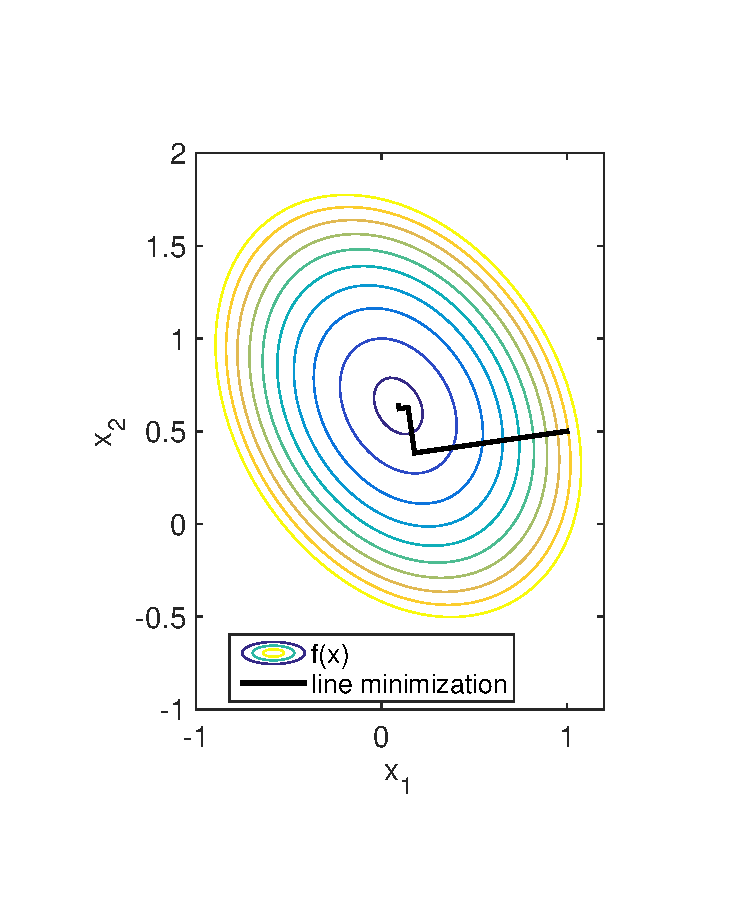
\includegraphics[width=2.5in]{08.matrix1/sd_min.pdf}
\caption{The steepest descent minimization of the 2D quadratic system (Example \ref{ex:sd_min}).  Fore steps are visible.  More steps (not visible in the plot) are needed to get sufficient accuracy.}
\label{fig:sd_min}
	\end{subfigure}
	\begin{subfigure}{0.45\textwidth}
		\centering
		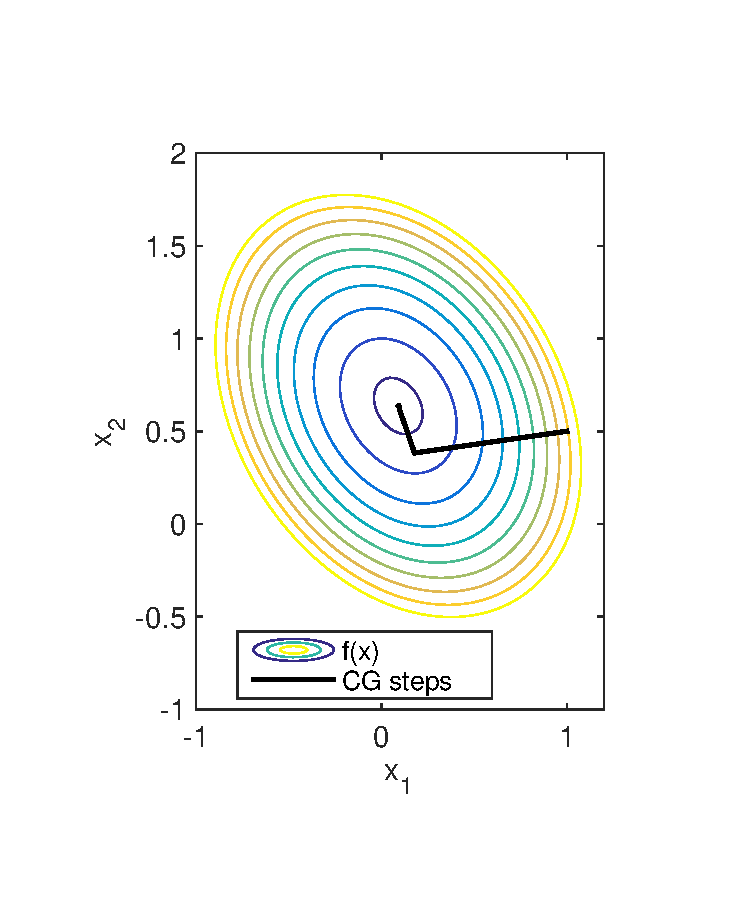
\includegraphics[width=2.5in]{08.matrix1/cg_min.pdf}
\caption{The conjugate gradient minimization of the 2D quadratic system (Example \ref{ex:cg_min}.  By construction, it needs only two steps to find the solution.}
\label{fig:cg_min}
	\end{subfigure}
\\
	\begin{subfigure}{4.5in}
		\centering
		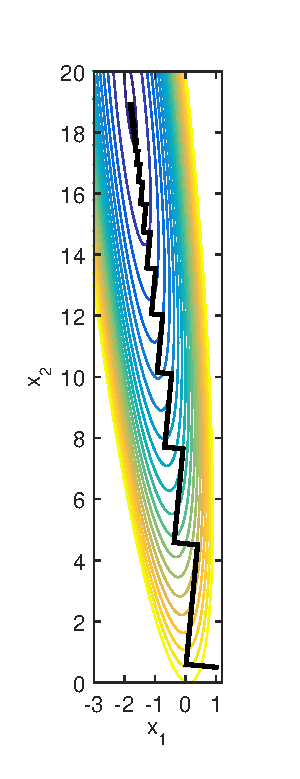
\includegraphics[angle=270, width=4in]{08.matrix1/sd_min_slow.pdf}
\caption{When the function has a narrow valley like this case, the steepest descent method takes a long zig-zag path, making it very inefficient.}
\label{fig:sd_min_slow}
\caption{Illustration of steepest descent/conjugate gradient methods.}
	\end{subfigure}
\end{figure}
\end{example}

\noindent
\subsection{Conjugate Gradient Method}

The steepest descent method becomes inefficient when the trajectory is trapped in a narrow valley as shown in Fig. \ref{fig:sd_min_slow}.
For a quadratic system \eqref{eq:cost_quadratic}, there is an algorithm called \textit{conjugate gradient} method\cite{cg_min} which find the solution in exactly $N$ iterations for $N$ dimensional quadratic system.  We again assume that $A$ is symmetric and positive definite.  The conjugate gradient method utilizes the geometry of quadratic system as summarized in Algorithm \ref{algo:conjugate-gradient}.

\begin{myalgobox}
   \Algorithm{Conjugate Gradient Method}\label{algo:conjugate-gradient}

   \medskip
   \begin{enumerate}
      \item Start with an initial guess $\vb{x}_0$ and $n=0$.
      \item Set the initial residual vector: $\vb{r}_0=\vb{b} - A \vb{x}_0$ 
      \item Set the initial conjugate direction: $\vb{p}_0 = \vb{r}_0$.
      \item Evaluate the step size: $\alpha = \displaystyle\frac{\vb{r}_n^\textsc{t} \vb{r}_n}{\vb{p}_n^\textsc{t} A \vb{p}_n}$.
      \item Update the point:  $\vb{x}_{n+1} = \vb{x}_n + \alpha \vb{p}_n$.
      \item Update the residual vector:  $\vb{r}_{n+1} = \vb{r}_n - \alpha A \vb{p}_n$.
      \item If $|\vb{r}_{n+1}| < \text{tolerance}$, $\vb{x}_{n+1}$ is the solution.  Otherwise continue.
      \item Evaluate the other step size: $\beta = \displaystyle\frac{\vb{r}_{n+1}^\textsc{t} \vb{r}_{n+1}}{\vb{r}_n^\textsc{t} \vb{r}_n}$.
      \item Update the conjugate vector: $\vb{p}_{n+1} = \vb{r}_{n+1} + \beta \vb{p}_n$.
      \item Increment $n$ and go to step 4.
\end{enumerate}

\end{myalgobox}


\bigskip
\begin{example}\label{ex:cg_min}

\medskip
\noindent
We solve the same problem as Example \ref{ex:sd_min} again but with the conjugate gradient method. Program \ref{prog:cg_min} implements the above Algorithm and solve the problem. Figure \ref{fig:cg_min} shows that two steps of line minimization hits the minimum as expected.  The solution is in a good agreement with the exact one.

\begin{mybox}
\small
\begin{verbatim}
Solution=(0.09089,0.63638)
\end{verbatim}
\normalsize
\end{mybox}
\end{example}


\noindent
\section{Applications in Physics}

\subsection{Multiloop circute: Kirchhoff rules}


\begin{minipage}{4in} 
\noindent
Find currents $I_i,\, i=1,2,3$ in the circuit shown in Figure.

\medskip
Applying the Kirchhoff rules, we find a set of equations for the currents
\begin{eqnarray*}
I_1 - I_2 - I_3 &=& 0 \\
3I_1 + 2 I_2 &=& 3 \\
-2 I_2 + 4 I_3 &=& 3\\
\end{eqnarray*}
\end{minipage}
\begin{minipage}{2.0in}
\begin{center}
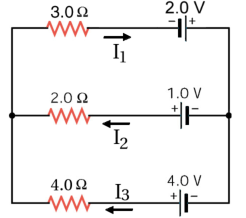
\includegraphics[width=1.7in]{08.matrix1/kirchhoff.pdf}\\
\end{center}
\end{minipage}

\noindent
or in a matrix form $A \vb{I}=\vb{b}$ with
\begin{equation*}
A = \begin{bmatrix} 1 & -1 & -1 \\ 3 & 2 & 0 \\ 0& -2 & 4\end{bmatrix}, \qquad 
\vb{b}=\begin{bmatrix} 0 \\ 3 \\ 3 \end{bmatrix}
\end{equation*}
The code used in Example \ref{ex:gaussian_elimination_pivot} can be used.  The answer is
$I_1=0.92308$ A, $I_2= 0.11538$ A, $I_3=0.80769$ A.
 
\subsection{Coupled Harmonic Oscillators in a Uniform Gravity}

\begin{minipage}{5.3in}
Four particles of mas $m_i$ ($i=1,\cdots, 4$) are linked by four springs and the whole system is hanged from the ceiling as shown in Figure. The natural length of the springs is $\ell_1=\ell_3=0.1\, m$, $\ell_2=\ell_4=0.2\,$ and their spring constants are
$k_1=k_4=100\, N/m$ and $k_2=k_3=150\, N/m$.  The mass of particles is $m_1=m_2=0.15\, kg$, $m_3=m_4=0.30\, kg$  We want to know the distance between particles when the system is at a mechanical equilibrium.
The force on each particles are given by
\begin{subequations}
\begin{eqnarray}
F_1 &=& k_1 x_1 - k_2 x_2 - m_1 g\\
F_2 &=& k_2 x_2 - k_3 x_3 - m_2 g\\
F_3 &=& k_3 x_3 - k_4 x_4 - m_3 g\\
F_4 &=& k_4 x_4 -m_2 g\, .
\end{eqnarray}
\end{subequations}
\end{minipage}
\hfill
\begin{minipage}{1in}
\hfill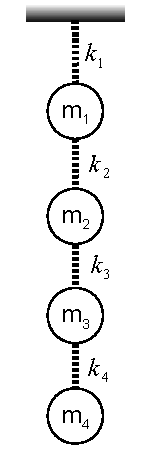
\includegraphics[width=0.6in]{08.matrix1/vertical_chain.pdf}
\end{minipage}

\bigskip
\noindent
where $x_i$ is the stretch of each spring from its natural length.  At the mechanical equilibrium, the force on each particle must vanish.  Hence, $F_i=0$ for all $i$.  Writing it in matrix form
$A \vb{x} = \vb{b}$,
\begin{equation}
A = \begin{bmatrix} 
k_1 & -k_2 &    0 &    0 \\
  0 &  k_2 & -k_3 &    0\\
  0 &    0 &  k_3 &  -k_4 \\
  0 &    0 &    0 &  k4
 \end{bmatrix}, \qquad
\vb{b} =\begin{bmatrix} m_1 g \\ m_2 g \\ m_3 g \\ m_4 g \end{bmatrix}
\end{equation}
The matrix is already upper triangular and thus we can solve it immediately using back substitution.  Taking into account the natural length, the distance between particles $i-1$ and $i$ is $d_{i-1,i}=\ell_i + x_i$.  We can use Program \ref{prog:triangular_matrix} to solve this problem.  The answer is $d_{12}=0.249000$, $d_{23}=0.139200$, $d_{34}=0.229400$.


\subsection{Determinant of Tree Graphs: Graham-Pollack theorem}

Consider a graph shown in Fig \ref{fig:tree-graph}.  This graph consist of $n=10$ vertices and 9 edges.   When there is no loop in it, the graph is called tree.   A tree of $n$ vertices has $n-1$ edges.
We consider distance between vertices.  The distance between vertices $v_2$ and $v_9$ is 3 since there are three edges between them.
The distance of between $v_i$ and $v_j$ forms a distance matrix $D_{ij}$.  The example graph shown in Fig \ref{fig:tree-graph} has a distance matrix
\begin{equation}
D=
\begin{bmatrix}
0 & 1 & 2 & 3 & 4 & 4 & 3 & 4 & 4 & 5 \\
1 & 0 & 1 & 2 & 3 & 3 & 2 & 3 & 3 & 4 \\
2 & 1 & 0 & 1 & 2 & 2 & 1 & 2 & 2 & 3 \\
3 & 2 & 1 & 0 & 1 & 1 & 2 & 3 & 3 & 4 \\
4 & 3 & 2 & 1 & 0 & 2 & 3 & 4 & 4 & 5 \\
4 & 3 & 2 & 1 & 2 & 0 & 3 & 4 & 4 & 5 \\
3 & 2 & 1 & 2 & 3 & 3 & 0 & 1 & 1 & 2 \\
4 & 3 & 2 & 3 & 4 & 4 & 1 & 0 & 2 & 3 \\
4 & 3 & 2 & 3 & 4 & 4 & 1 & 2 & 0 & 1 \\
5 & 4 & 3 & 4 & 5 & 5 & 2 & 3 & 1 & 0
\end{bmatrix}
\end{equation}
In 1971, Graham and Pollak obtained a remarkable formula\cite{graham-pollak,graham-pollak2}
\begin{equation}
\det(D) = -(n-1) (-2)^{n-2}
\end{equation}
which is independent of the structure of the tree.  For the above distance matrix, $\det(D)=-9 \cdot (-2)^8 = -2304$.  We now check it by numerical calculation.  Program \ref{prog:graham-pollak} calculates the determinant of the distance matrix using Gaussian elimination with partial pivoting. The output is
\begin{mybox}
\small
\begin{verbatim}
Gaussian Elimination: -2304.000000
       Graham-Pollak: -2304.000000
\end{verbatim}
\normalsize
\end{mybox}
The formula works!

\begin{figure}
\centering
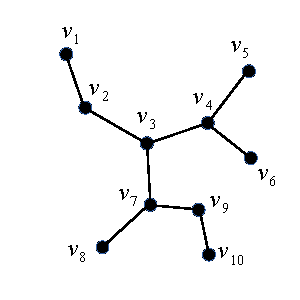
\includegraphics[width=2.0in]{08.matrix1/tree-graph.pdf}
\caption{A small example of tree graph.  It has 10 vertices and 9 edges.However, there is no loop.}
\label{fig:tree-graph}
\end{figure}
\newpage
\section{Problems}

\begin{enumerate}[labelwidth=0.5cm,labelindent=0cm,leftmargin=*,label=\bfseries \thechapter.\arabic*,align=left]

\item \textbf{Orthogoinal matrices}\label{pr:rotation}

A rotation matrix $R$ rotates points in a coordinate space.  Accordingly, any vector $\vb{a}$ is rotated as  $\vb{b} = R \vb{a}$. Since rotation does not changes the norm of vector, $b^\textsc{t} b = a^\textsc{t} R^\textsc{t} R a = a^\textsc{t} a$ where $\textsc{t}$ indicates transpose.  Hence, $R^\textsc{t} R = I$ where $I$ is the identity matrix.  This means the rotation matrix is an orthogonal matrix defined by $R^{-1} = R^\textsc{t}$.  A rotation of $-74^\circ$ around the axes (-1/3,2/3,2/3) is given by a rotation matrix
\begin{equation}
R = \begin{bmatrix} 0.36&0.48&-0.80\\-0.80&0.60&0\\0.48&0.64&0.60 \end{bmatrix}.
\end{equation}
Show that this matrix is indeed orthogonal by comparing $R^{-1}$ and $R^\textsc{t}$.  You may use build-in functions in MATLAB or Numpy.

\item 
\begin{minipage}[t]{4in}
Three particles are chained by four springs as shown in Fig.  Two springs at the ends are fixed to the walls.  The walls are separated by distance $d=8$.
The natural length of the springs are $\ell_1=\ell_3=1$, $\ell_2=\ell_4=2$ and their spring constants are
$k_1=k_4=2$ and $k_2=k_3=4$.
Let $d_i$ be the length of the $i$-th spring.  The potential energy of the system is defined by $U=\sum_{i} \frac{1}{2} k_i (d_i - \ell_i)^2$.
Letting the position of the particles $x_i,  i=1,\cdots, 4$.  
\end{minipage}
\begin{minipage}{2.3in}
   
   \vspace{1in}
   \begin{center}
      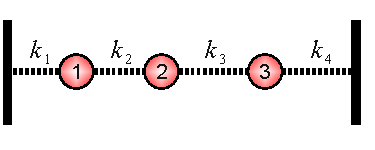
\includegraphics[width=2in]{08.matrix1/spring_chain.pdf}
   \end{center}
\end{minipage}
\begin{equation}\label{eq:coupled_osc_potential}
   U = \frac{k_1}{2} (x_1-\ell_1)^2 + \frac{k_2}{2} (x_2-x_1-\ell_2)^2 + \frac{k_3}{2} (x_3-x_2-\ell_3)^2+\frac{k_4}{2} (d-x_3-\ell_4)^2
\end{equation}
Find the length of the springs at mechanical equilibrium. Yu may use built-in functions such as linsolve() in MATLAB.

[Solve $\pdv{x_1} U(x_1,x_2,x_3) = 0$, $\pdv{x_2} U(x_1,x_2,x_3) = 0$, and $\pdv{x_3} U(x_1,x_2,x_3) = 0$ for $x_1$, $x_2$, and $x_3$.]
\end{enumerate}

\vfill

\newpage
\section*{MATLAB Source Codes}
\addcontentsline{toc}{section}{\protect\numberline{}MATLAB Source Codes}

\bigskip
\noindent
\program
\label{prog:triangular_matrix}
\footnotesize
\begin{verbatim}
%**************************************************************************
%*     Example  8.1                                                       *
%*     filename: ch08pr01.m                                               *
%*     program listing number: 8.1                                        *
%*                                                                        *
%*     This program checks the properties of triangular matrices.         *
%*                                                                        *
%*     Programed by Ryoichi Kawai for Computational Physics Course.       *
%*     Last modification:  01/31/2015.                                    *
%**************************************************************************
clear all;

% define matrices A and B
A=[[2, 0, 0];[-1,1,0];[3,2,-1]]
B=[[1, 0, 0];[2,4,0];[-1,-2,3]]

C=A*B;
fprintf('Mutilication: A*B\n')
% MATLAB print column first. Thus you need to print its transpose
fprintf('%3d %3d %3d\n',C')
fprintf('\nInverse of A\n')
D=inv(A);
fprintf('%15.4e %15.4e %15.4e\n',D')

E1=A(1,1)*A(2,2)*A(3,3);
E2=det(A);
fprintf('\nProducts of the diagonal elements = %d\n',E1)
fprintf('Determinant by MATLAB = %d\n',E2)
\end{verbatim}
\normalsize

\ruleend

\bigskip
\noindent
\program
\label{prog:triangular_matrix2}
\footnotesize
\begin{verbatim}
%**************************************************************************
%*     Example  8.2                                                       *
%*     filename: ch08pr02.m                                               *
%*     program listing number: 8.2                                        *
%*                                                                        *
%*     This program solves a upper-triangular linear equation with        *
%*     the backsubstitution method.                                       *
%*                                                                        *
%*     Programed by Ryoichi Kawai for Computational Physics Course.       *
%*     Last modification:  10/13/2013.                                    *
%**************************************************************************
clear all;

% define matrix A and vector b
A=[[3, -1, 4];[0,2,-1];[0,0,2]];
b=[-1;-2;4];

% backsubstitution
for i=3:-1:1
    Ax=0;
    for j=i+1:3
        Ax = Ax+A(i,j)*x(j);
    end
    x(i) = (b(i)-Ax)/A(i,i);
end

fprintf('x=%.1f, y=%.1f, z=%.1f\n',x)
\end{verbatim}
\normalsize

\ruleend

\bigskip
\noindent
\program
\label{prog:gaussian_elimination}
\footnotesize
\begin{verbatim}
%**************************************************************************
%*     Example  8.3                                                       *
%*     filename: ch08pr03.m                                               *
%*     program listing number: 8.3                                        *
%*                                                                        *
%*     This program solves a simple linear equation with the Gaussian     *
%*     eliminationa and backsubstitution methods.                         *
%*                                                                        *
%*     Programed by Ryoichi Kawai for Computational Physics Course.       *
%*     Last modification:  10/13/2013.                                    *
%**************************************************************************
clear all;

% Set a linear equation
N=3;
A=[[3,-1,4];[2,0,-1];[0,3,2]];
b=[2;-1;3];

%forward elimination
for n=1:N-1
    for i=n+1:N
        M=-A(i,n)/A(n,n);
        A(i,n+1:N)=M*A(n,n+1:N)+A(i,n+1:N);
        b(i)=M*b(n)+b(i);
    end
    A(n+1,n)=0;  
end

% backsubstitution
for i=3:-1:1
    Ax=0;
    for j=i+1:3
        Ax = Ax+A(i,j)*x(j);
    end
    x(i) = (b(i)-Ax)/A(i,i);
end

% result
fprintf('\nA=\n')
fprintf('%8.5f  %8.5f  %8.5f\n',A')
fprintf('\nb=\n')
fprintf('%8.5f\n',b)
fprintf('\nx=\n')
fprintf('%8.5f\n',x)
\end{verbatim}
\normalsize

\ruleend

\bigskip
\noindent
\program
\label{prog:gaussian_elimination_pivot}
\footnotesize
\begin{verbatim}
%**************************************************************************
%*     Example  8.4                                                       *
%*     filename: ch08pr04.m                                               *
%*     program listing number: 8.4                                        *
%*                                                                        *
%*     This program solves a simple linear equation with the Gaussian     *
%*     elimination with partial pivoting and backsubstitution methods.    *
%*                                                                        *
%*     Programed by Ryoichi Kawai for Computational Physics Course.       *
%*     Last modification:  10/13/2013.                                    *
%**************************************************************************
clear all;

% Set a linear equation
N=3;
A=[[3,-1,4];[2,0,-1];[0,3,2]];
b=[2;-1;3];
P=eye(N,N);  % permutation matrix is initially an identity matrix

% Find scale factors
for i=1:N
    S(i)=max(A(i,:));
end

for n=1:N-1
    % Look for the pivot row
    j=n;
    Amax=abs(A(n,n)/S(n));
    for i=n:N
        AS=abs(A(i,n)/S(i));
        if AS > Amax
            j=i;
            Amax = AS;
        end
    end
    % Carry out pivoting
    if j ~= n
        for i=n:N
            TMP=A(n,i);
            A(n,i)=A(j,i);
            A(j,i)=TMP;
        end
        TMP=b(n);
        b(n)=b(j);
        b(j)=TMP;
        % Record the permutation
        P(n,n)=0; P(j,j)=0;
        P(n,j)=1; P(j,n)=1;
    end
    % Gaussian elimination
    for i=n+1:N
        M=-A(i,n)/A(n,n);
        A(i,n+1:N)=M*A(n,n+1:N)+A(i,n+1:N);
        b(i)=M*b(n)+b(i);
    end
    A(n+1,n)=0;  
end

% backsubstitution
for i=3:-1:1
    Ax=0;
    for j=i+1:3
        Ax = Ax+A(i,j)*x(j);
    end
    x(i) = (b(i)-Ax)/A(i,i);
end

% result
fprintf('\nA=\n')
fprintf('%8.5f  %8.5f  %8.5f\n',A')
fprintf('\nb=\n')
fprintf('%8.5f\n',b)
fprintf('\nP=\n')
fprintf('%i  %i  %i\n',P')
fprintf('\nx=\n')
fprintf('%8.5f\n',x)
\end{verbatim}
\normalsize

\ruleend

\bigskip
\noindent
\program
\label{prog:matrix_inverse}
\footnotesize
\begin{verbatim}
%**************************************************************************
%*     Example  8.6                                                       *
%*     filename: ch08pr05.m                                               *
%*     program listing number: 8.5                                        *
%*                                                                        *
%*     This program calculates the inverse of a given matrix using        *
%*     Gaussi-Jordin methods.                                             *
%*                                                                        *
%*     Programed by Ryoichi Kawai for Computational Physics Course.       *
%*     Last modification:  10/13/2013.                                    *
%**************************************************************************
clear all;

% Set a linear equation
N=3;
A0=[[3,-1,4];[2,0,-1];[0,3,2]];
A=A0; % keep the original matrix
b=eye(N,N);

% scale factors
for i=1:N
    S(i)=max(A(i,:));
end

for n=1:N-1
    % Look for the pivot row
    j=n;
    Amax=abs(A(n,n)/S(n));
    for i=n:N
        AS=abs(A(i,n)/S(i));
        if AS > Amax
            j=i;
            Amax = AS;
        end
    end
    % Carry out pivoting
    if j ~= n
        for i=n:N
            TMP=A(n,i);
            A(n,i)=A(j,i);
            A(j,i)=TMP;
        end
        TMP2(1:N) = b(n,:);
        b(n,:)=b(j,:);
        b(j,:)=TMP2(1:N);
    end
    % Gaussian elimination
    for i=n+1:N
        M=-A(i,n)/A(n,n);
        A(i,n+1:N)=M*A(n,n+1:N)+A(i,n+1:N);
        b(i,:)=M*b(n,:)+b(i,:);
    end
    A(n+1,n)=0;  
end

% backsubstitution
for i=3:-1:1
    Ax(1:N)=0;
    for j=i+1:3
        for k=1:N
            Ax(k) = Ax(k)+A(i,j)*x(j,k);
        end
    end
    for j=1:N
        x(i,j) = (b(i,j)-Ax(j))/A(i,i);
    end
end

% result
fprintf('\nInvers of A=\n')
fprintf('%8.5f  %8.5f  %8.5f\n',x)
fprintf('\nA A^(-1)=\n')
fprintf('%8.5f  %8.5f  %8.5f\n',A0*x)
\end{verbatim}
\normalsize

\ruleend

\bigskip
\noindent
\program
\label{prog:LU}
\footnotesize
\begin{verbatim}
%**************************************************************************
%*     Example  8.7                                                       *
%*     filename: ch08pr06.m                                               *
%*     program listing number: 8.6                                        *
%*                                                                        *
%*     This program solves a simple linear equation with LU decomposition.*
%*     MATLAB function lu() is used.                                      *
%*                                                                        *
%*     Programed by Ryoichi Kawai for Computational Physics Course.       *
%*     Last modification:  10/13/2013.                                    *
%**************************************************************************
clear all;

% Define a matrix
A=[[3, -1, 4];[2, 0, -1];[0, 3, 2]];
b=[2;-1;3];

% LU dcomposition
[L U P]=lu(A);

% Rcover the original matrix
S=P*L*U;

% Show the results
fprintf('\nA (Original Matrix)\n')
fprintf('%8.5f  %8.5f  %8.5f\n',A')
fprintf('\nL (Lower Triangular Matrix)\n')
fprintf('%8.5f  %8.5f  %8.5f\n',L')
fprintf('\nU (Upper Triangular Matrix)\n')
fprintf('%8.5f  %8.5f  %8.5f\n',U')
fprintf('\nP (Permutation Matrix)\n')
fprintf('%i  %i  %i\n',P')
fprintf('\nP*L*U\n')
fprintf('%8.5f  %8.5f  %8.5f\n',S')

b = P*b;
% forward substition
for i=1:3
    Ly=0;
    for j=1:i-1
        Ly = Ly+L(i,j)*y(j);
    end
    y(i) = (b(i)-Ly)/L(i,i);
end

% backsubstitution
for i=3:-1:1
    Ux=0;
    for j=i+1:3
        Ux = Ux+U(i,j)*x(j);
    end
    x(i) = (y(i)-Ux)/U(i,i);
end

fprintf('\nx=%.5f,  y=%.5f, z=%.5f\n',x)
\end{verbatim}
\normalsize

\ruleend

\bigskip
\noindent
\program
\label{prog:tridiagonal}
\footnotesize
\begin{verbatim}
%**************************************************************************
%*     Example  8.9                                                       *
%*     filename: ch08pr07.m                                               *
%*     program listing number: 8.7                                        *
%*                                                                        *
%*     This program solves a tridiagonal system with backward elimination.*
%*     Then, find solution by forward substitution.                       *
%*                                                                        *
%*     Programed by Ryoichi Kawai for Computational Physics Course.       *
%*     Last modification:  02/01/2015.                                    *
%**************************************************************************
clear all

% Define matrices. No need to use the full matrix.
d=[2,3,4,3]; % diagonal elements
u=[2,3,3,0]; % above diagonal
l=[0,2,3,3]; % below diagonal
b=[1,2,3,4]; % right hand side

% Calculation of determinant
D(1)=d(1);
D(2)=d(2)*D(1)-l(1)*u(1);
for i=3:4
    D(i)=d(i)*D(i-1)-l(i-1)*u(i-1)*D(i-2);
end

fprintf('Determinant %d\n',D(4))
if D(4) == 0
    fprintf('Singular')
    stop
end

% Decomposition by backword elimination
Y(3)=-l(4)/d(4);
Z(3)= b(4)/d(4);
for i=3:-1:2
    Y(i-1)=-l(i)/(d(i)+u(i)*Y(i));
    Z(i-1)=(b(i)-u(i)*Z(i))/(d(i)+u(i)*Y(i));
end

% Forward substitution
x(1)=(b(1)-u(1)*Z(1))/(d(1)+u(1)*Y(1));
for i=1:3
    x(i+1)=Y(i)*x(i)+Z(i);
end

% Answer
fprintf('x= %f %f %f %f\n',x)

% Check the errors. 
s(1)=d(1)*x(1)+u(1)*x(2)-b(1);
s(2)=l(2)*x(1)+d(2)*x(2)+u(2)*x(3)-b(2);
s(3)=l(3)*x(2)+d(3)*x(3)+u(3)*x(4)-b(3);
s(4)=l(4)*x(3)+d(4)*x(4)-b(4);
fprintf('Error= %e %e %e %e\n',s)
\end{verbatim}
\normalsize


\ruleend

\bigskip
\noindent
\program
\label{prog:graham-pollak}
\footnotesize
\begin{verbatim}
%**************************************************************************
%*     Section  8.6.3                                                     *
%*     filename: ch08pr08.m                                               *
%*     program listing number: 8.8                                        *
%*                                                                        *
%*     This program calculate the determinant of distance matrix for      *
%*     a tree graph using Gaussian elimination with partial pivoting.     *
%*                                                                        *
%*     Programed by Ryoichi Kawai for Computational Physics Course.       *
%*     Last modification:  02/01/2015.                                    *
%**************************************************************************
clear all;

% Set a linear equation
N=10;
A=[[0 , 1 , 2 , 3 , 4 , 4 , 3 , 4 , 4 , 5 ];...
   [1 , 0 , 1 , 2 , 3 , 3 , 2 , 3 , 3 , 4 ];...
   [2 , 1 , 0 , 1 , 2 , 2 , 1 , 2 , 2 , 3 ];...
   [3 , 2 , 1 , 0 , 1 , 1 , 2 , 3 , 3 , 4 ];...
   [4 , 3 , 2 , 1 , 0 , 2 , 3 , 4 , 4 , 5 ];...
   [4 , 3 , 2 , 1 , 2 , 0 , 3 , 4 , 4 , 5 ];...
   [3 , 2 , 1 , 2 , 3 , 3 , 0 , 1 , 1 , 2 ];...
   [4 , 3 , 2 , 3 , 4 , 4 , 1 , 0 , 2 , 3 ];...
   [4 , 3 , 2 , 3 , 4 , 4 , 1 , 2 , 0 , 1 ];...
   [5 , 4 , 3 , 4 , 5 , 5 , 2 , 3 , 1 , 0 ]];

P=eye(N,N);  % permutation matrix is initially an identity matrix

% Find scale factors
for i=1:N
    S(i)=max(A(i,:));
end

for n=1:N-1
    % Look for the pivot row
    j=n;
    Amax=abs(A(n,n)/S(n));
    for i=n:N
        AS=abs(A(i,n)/S(i));
        if AS > Amax
            j=i;
            Amax = AS;
        end
    end
    % Carry out pivoting
    if j ~= n
        for i=n:N
            TMP=A(n,i);
            A(n,i)=A(j,i);
            A(j,i)=TMP;
        end
        % Record the permutation
        P(n,n)=0; P(j,j)=0;
        P(n,j)=1; P(j,n)=1;
    end
    % Gaussian elimination
    for i=n+1:N
        M=-A(i,n)/A(n,n);
        A(i,n+1:N)=M*A(n,n+1:N)+A(i,n+1:N);
    end
    A(n+1,n)=0;  
end

p=sum(sum(P))
D=(-1)^p;
for i=1:10
    D=D*A(i,i);
end
D_GP=-(N-1)*(-2)^(N-2);
fprintf('Gaussian Elimination: %f\n',D)
fprintf('       Graham-Pollak: %f\n',D_GP)
\end{verbatim}
\normalsize

\ruleend

\bigskip
\noindent
\program
\label{prog:sd_min}
\footnotesize
\begin{verbatim}
%**************************************************************************
%*     Example  8.10                                                      *
%*     filename: ch08pr09.m                                               *
%*     program listing number: 8.9                                        *
%*                                                                        *
%*     This program solves a 2x2 linear equation by the steepest descent  *
%*     minimization.                                                      *
%*                                                                        *
%*     Programed by Ryoichi Kawai for Computational Physics Course.       *
%*     Last modification:  10/13/2013.                                    *
%**************************************************************************
clear all;
A=[[4,1];[1,3]];
b=[1;2];
c=[-0.65,  -0.5, -0.3,  -0.1, 0.1,  0.3, 0.5, 0.7, 0.9, 1.1];
tol = 1e-8;

% contour plot of the cost function
x=linspace(-1,1.2);
y=linspace(-1,2);
[X,Y]=meshgrid(x,y);
N=size(X,2);
M=size(Y,2);
for i=1:N
    for j=1:M
        Z(i,j) = 0.5*(X(i,j)^2*A(1,1)+(A(1,2)+A(2,1))*X(i,j)*Y(i,j)...
                 +A(2,2)*Y(i,j)^2) - X(i,j)*b(1)-Y(i,j)*b(2);
    end
end

contour(X,Y,Z,c);
hold on

% steepest descent with line minimization
n=1;
x=[1;0.5]; % starting point
u(1)=x(1);
v(1)=x(2);
g = A*x-b;
gg=g'*g;
while abs(gg)>tol
    n=n+1;
    lambda = gg/(g'*A*g);
    x = x - lambda * g;
    u(n)=x(1);
    v(n)=x(2);
    g = A*x-b;
    gg = g'*g;
end

fprintf('Solution=(%.5f,%.5f)\n',x)

p=plot(u,v);
set(p,'linewidth',2,'color','black')
axis equal tight
xlabel(texlabel('x_1'),'fontsize',14)
ylabel(texlabel('x_2'),'fontsize',14)

hold off
\end{verbatim}
\normalsize


\ruleend

\bigskip
\noindent
\program
\label{prog:cg_min}
\footnotesize
\begin{verbatim}
%**************************************************************************
%*     Example  8.11                                                      *
%*     filename: ch08pr10.m                                               *
%*     program listing number: 8.10                                       *
%*                                                                        *
%*     This program solves a 2x2 linear equation by the conjugate         *
%*     gradient minimization.                                             *
%*                                                                        *
%*     Programed by Ryoichi Kawai for Computational Physics Course.       *
%*     Last modification:  10/13/2013.                                    *
%**************************************************************************
clear all;
A=[[4,1];[1,3]];
b=[1;2];
c=[-0.65,  -0.5, -0.3,  -0.1, 0.1,  0.3, 0.5, 0.7, 0.9, 1.1];
tol = 1e-8;

% contour plot of the cost function
x=linspace(-1,1.2);
y=linspace(-1,2);
[X,Y]=meshgrid(x,y);
N=size(X,2);
M=size(Y,2);
for i=1:N
    for j=1:M
        Z(i,j) = 0.5*(X(i,j)^2*A(1,1)+(A(1,2)+A(2,1))*X(i,j)*Y(i,j)...
                 +A(2,2)*Y(i,j)^2) - X(i,j)*b(1)-Y(i,j)*b(2);
    end
end

contour(X,Y,Z,c);
hold on

% conjugate gradient method
n=1;
x=[1;0.5]; % starting point
u(1)=x(1);
v(1)=x(2);
r=b- A*x;
p=r;
rr=r'*r;
while abs(rr)>tol
    n=n+1;
    alpha = rr/(r'*A*r);
    x = x + alpha*p;
    u(n)=x(1);
    v(n)=x(2);
    r1=b-A*x;
    rr1=r1'*r1;
    beta=rr1/rr;
    r=r1;
    rr=rr1;
    p=r+beta*p;
end

fprintf('Solution=(%.5f,%.5f)\n',x)

p=plot(u,v);
set(p,'linewidth',2,'color','black')
axis equal tight
xlabel(texlabel('x_1'),'fontsize',14)
ylabel(texlabel('x_2'),'fontsize',14)
legend('f(x)','CG steps');
hold off
\end{verbatim}
\normalsize

\ruleend

\bigskip
\noindent
\section*{Python Source Codes}
\addcontentsline{toc}{section}{\protect\numberline{}Python Source Codes}
\setcounter{program}{0}

\bigskip
\noindent
\program
\footnotesize
\begin{verbatim}
#!/usr/bin/env python3
# -*- coding: utf-8 -*-
"""
%**************************************************************************
%*     Example  8.1                                                       *
%*     filename: ch08pr01.m                                               *
%*     program listing number: 8.1                                        *
%*                                                                        *
%*     This program checks the properties of triangular matrices.         *
%*                                                                        *
%*     Programed by Ryoichi Kawai for Computational Physics Course.       *
%*     Last modification:  01/31/2015.                                    *
%**************************************************************************
"""
import numpy as np

# define matrices A and B (do not use array)
A=np.matrix([[2, 0, 0],[-1,1,0],[3,2,-1]])
B=np.matrix([[1, 0, 0],[2,4,0],[-1,-2,3]])

print("A*B")
print(A*B)

print('\nInverse of A')
print(np.linalg.inv(A))

print("\nDeterminant of A={0:7.5f}".format(np.linalg.det(A)))
\end{verbatim}

\ruleend

\bigskip
\noindent
\program
\footnotesize
\begin{verbatim}
#!/usr/bin/env python3
# -*- coding: utf-8 -*-
"""
%**************************************************************************
%*     Example  8.2                                                       *
%*     filename: ch08pr02.py                                              *
%*     program listing number: 8.2                                        *
%*                                                                        *
%*     This program solves a upper-triangular linear equation with        *
%*     the backsubstitution method.                                       *
%*                                                                        *
%*     Programed by Ryoichi Kawai for Computational Physics Course.       *
%*     Last modification:  02/06/2017.                                    *
%**************************************************************************
"""
import numpy as np

# define matrix A and vector b
A=np.matrix([[3, -1, 4],[0,2,-1],[0,0,2]])
b=np.matrix([[-1],[-2],[4]])
x=b
# backsubstitution
for i in range(2,-1,-1):
    Ax=0.0
    for j in range(i+1,3):
        Ax = Ax+A[i,j]*x[j]

    x[i] = (b[i]-Ax)/A[i,i]

print(x)
\end{verbatim}

\ruleend

\bigskip
\noindent
\program
\footnotesize
\begin{verbatim}
#!/usr/bin/env python3
# -*- coding: utf-8 -*-
"""
%**************************************************************************
%*     Example  8.3                                                       *
%*     filename: ch08pr03.py                                              *
%*     program listing number: 8.3                                        *
%*                                                                        *
%*     This program solves a simple linear equation with the Gaussian     *
%*     eliminationa and backsubstitution methods.                         *
%*                                                                        *
%*     Programed by Ryoichi Kawai for Computational Physics Course.       *
%*     Last modification:  02/06/2017.                                    *
%**************************************************************************
"""
import numpy as np

# Set a linear equation
N=3;
A=np.matrix([[3.,-1.,4.],[2.,0.,-1.],[0.,3.,2.]])
b=np.matrix.transpose(np.matrix([2.,-1.,3.]))
x=np.matrix.transpose(np.matrix(np.zeros(N)))

#forward elimination
for n in range(0,N-1):
  
    for i in range(n+1,N):
        M=-A[i,n]/A[n,n]
        A[i,n+1:N]=M*A[n,n+1:N]+A[i,n+1:N]
        b[i]=M*b[n]+b[i]

    A[n+1,n]=0.0 


# backsubstitution
for i in range(2,-1,-1):
    Ax=0.0
    for j in range(i+1,3):
        Ax = Ax+A[i,j]*x[j]

    x[i] = (b[i]-Ax)/A[i,i]


# result
print('\nA=\n')
print(A)
print('\nb=\n')
print(b)
print('\nx=\n')
print(x)
\end{verbatim}

\ruleend

\bigskip
\noindent
\program
\footnotesize
\begin{verbatim}
#!/usr/bin/env python3
# -*- coding: utf-8 -*-
"""
%**************************************************************************
%*     Example  8.4                                                       *
%*     filename: ch08pr04.pu                                              *
%*     program listing number: 8.4                                        *
%*                                                                        *
%*     This program solves a simple linear equation with the Gaussian     *
%*     elimination with poartial pivoting and backsubstitution methods.   *
%*                                                                        *
%*     Programed by Ryoichi Kawai for Computational Physics Course.       *
%*     Last modification:  02/08/2017.                                    *
%**************************************************************************
"""

# Set a linear equation
N=3;
A=np.matrix([[3.,-1.,4.],[2.,0.,-1.],[0.,3.,2.]])
b=np.matrix.transpose(np.matrix([2.,-1.,3.]))
x=np.matrix.transpose(np.matrix(np.zeros(N)))
# permutation matrix must be initially an identity matrix
P=np.matrix(np.identity(3,dtype=int))  
S=np.zeros(3)

# Find scale factors
for i in range(0,N):
    S[i]=A[i,:].max()


for n in range(0,N-1):
    # Look for the pivot row
    j=n
    Amax=abs(A[n,n]/S[n])
    for i in range(n,N):
        AS=abs(A[i,n]/S[i])
        if AS > Amax:
            j=i
            Amax = AS

    # Carry out pivoting
    if j != n :
        for i in range(n,N) :
            TMP=A.item(n,i)
            A[n,i]=A.item(j,i)
            A[j,i]=TMP

        TMP=b.item(n)
        b[n]=b.item(j)
        b[j]=TMP
        # Record the permutation
        P[n,n]=P[j,j]=0
        P[n,j]=P[j,n]=1

    # Gaussian elimination
    for i in range(n+1,N):
        M=-A[i,n]/A[n,n]
        A[i,n+1:N]=M*A[n,n+1:N]+A[i,n+1:N]
        b[i]=M*b[n]+b[i]

    A[n+1,n]=0.0  


# backsubstitution
for i in range(2,-1,-1):
    Ax=0.0
    for j in range(i+1,3):
        Ax = Ax+A[i,j]*x[j]

    x[i] = (b[i]-Ax)/A[i,i]

# result
print('\nA=\n')
print(A)
print('\nb=\n')
print(b)
print('\nP=\n')
print(P)
print('\nx=\n')
print(x)
\end{verbatim}

\ruleend

\bigskip
\noindent
\program
\footnotesize
\begin{verbatim}
#!/usr/bin/env python3
# -*- coding: utf-8 -*-
"""
%**************************************************************************
%*     Example  8.5                                                       *
%*     filename: ch08pr05.py                                              *
%*     program listing number: 8.5                                        *
%*                                                                        *
%*     This program calculates the inverse of a given matrix using        *
%*     Gaussi-Jordin methods.                                             *
%*                                                                        *
%*     Programed by Ryoichi Kawai for Computational Physics Course.       *
%*     Last modification:  02/08/2017.                                    *
%**************************************************************************
"""
import numpy as np

# Set a linear equation
N=3
A0=np.matrix([[3.,-1.,4.],[2.,0.,-1.],[0.,3.,2.]])
A=np.identity(N)
A[:,:]=A0[:,:]
b=np.matrix(np.identity(N))  # permutation matrix is initially an identity matrix
x=np.matrix(np.identity(N))
S=np.zeros(N)
TMP2=np.zeros(N)

# scale factors
for i in range(0,N): 
    S[i]=A[i,:].max()


for n in range(0,N-1):
    # Look for the pivot row
    j=n
    Amax=abs(A[n,n]/S[n])
    for i in range(n,N):
        AS=abs(A[i,n]/S[i])
        if AS > Amax:
            j=i
            Amax = AS

    # Carry out pivoting
    if j != n:
        for i in range(n,N): 
            TMP=A[n,i]
            A[n,i]=A[j,i]
            A[j,i]=TMP

        TMP2[:]=b[n,:]
        b[n,:]=b[j,:]
        b[j,:]=TMP2[:]

    # Gaussian elimination
    for i in range(n+1,N): 
        M=-A[i,n]/A[n,n]
        A[i,n+1:N]=M*A[n,n+1:N]+A[i,n+1:N]
        b[i,:]=M*b[n,:]+b[i,:]

    A[n+1,n]=0.0  

# backsubstitution
Ax=np.zeros(N)
for i in range(N-1,-1,-1):
    Ax=np.zeros(N)
    for j in range(i+1,N):
        for k in range(0,N):
            Ax[k] = Ax[k]+A.item(i,j)*x[j,k]

    x[i,:] = (b[i,:]-Ax[:])/A[i,i]

# result
print('\nInvers of A=')
print(x)
print('\nA A^(-1)=')
print(A0*x)
\end{verbatim}

\ruleend

\bigskip
\noindent
\program
\footnotesize
\begin{verbatim}
#!/usr/bin/env python3
# -*- coding: utf-8 -*-
"""
%**************************************************************************
%*     Example  8.6                                                       *
%*     filename: ch08pr06.py                                              *
%*     program listing number: 8.6                                        *
%*                                                                        *
%*     This program solves a simple linear equation with LU decomposition.*
%*     MATLAB function lu() is used.                                      *
%*                                                                        *
%*     Programed by Ryoichi Kawai for Computational Physics Course.       *
%*     Last modification:  02/08/2017.                                    *
%**************************************************************************
"""

import numpy as np
import scipy.linalg as la

# Define a matrix
A=np.matrix([[3., -1., 4.],[2., 0., -1.],[0., 3., 2.]])
b=np.matrix([2.,-1.,3.]).transpose()
x=np.matrix(np.zeros(3)).transpose()
y=np.matrix(np.zeros(3)).transpose()

# LU dcomposition
P, L, U = la.lu(A)
P=np.matrix(P)
U=np.matrix(U)
L=np.matrix(L)

# Rcover the original matrix
S=P*L*U
# Show the results
print('\nA (Original Matrix)')
print(A)
print('\nL (Lower Triangular Matrix)')
print(L)
print('\nU (Upper Triangular Matrix)')
print(U)
print('\nP (Permutation Matrix)')
print(P)
print('\nP*L*U')
print(S)

b = P*b
# forward substition
for i in range(0,3):
    Ly=0.0
    for j in range(0,i):
        Ly = Ly+L[i,j]*y[j]

    y[i] = (b[i]-Ly)/L[i,i]

# backsubstitution
for i in range(2,-1,-1):
    Ux=0.0
    for j in range(i+1,3):
        Ux = Ux+U[i,j]*x[j]

    x[i] = (y[i]-Ux)/U[i,i]

print('\nSolution x')
print(x)
\end{verbatim}

\ruleend

\bigskip
\noindent
\program
\footnotesize
\begin{verbatim}
#!/usr/bin/env python3
# -*- coding: utf-8 -*-
"""
%**************************************************************************
%*     Example  8.7                                                       *
%*     filename: ch08pr07.py                                              *
%*     program listing number: 8.7                                        *
%*                                                                        *
%*     This program solves a tridiagonal system with backward elimination.*
%*     Then, find solution by forward substitution.                       *
%*                                                                        *
%*     Programed by Ryoichi Kawai for Computational Physics Course.       *
%*     Last modification:  02/08/2017.                                    *
%**************************************************************************
"""
import numpy as np

# Define matrices. No need to use the full matrix.
d=[2,3,4,3] # diagonal elements
u=[2,3,3,0] # above diagonal
l=[0,2,3,3] # below diagonal
b=[1,2,3,4] # right hand side
D = np.zeros(4)
Y = np.zeros(4)
Z = np.zeros(4)
s = np.zeros(4)
x = np.zeros(4)
# Calculation of determinant
D[0]=d[0]
D[1]=d[1]*D[0]-l[0]*u[0]
for i in range(2,4):
    D[i]=d[i]*D[i-1]-l[i-1]*u[i-1]*D[i-2]


print('Determinant {0:8.3f}='.format(D[3]))
if D[3] == 0:
    exit('Singular')

# Decomposition by backword elimination
Y[2]=-l[3]/d[3]
Z[2]= b[3]/d[3]
for i in range(2,0,-1):
    Y[i-1]=-l[i]/(d[i]+u[i]*Y[i])
    Z[i-1]=(b[i]-u[i]*Z[i])/(d[i]+u[i]*Y[i])


# Forward substitution
x[0]=(b[0]-u[0]*Z[0])/(d[0]+u[0]*Y[0])
for i in range(0,3):
    x[i+1]=Y[i]*x[i]+Z[i]

# Answer
print('Solution x')
print(x)

# Check the errors. 
s[0]=          d[0]*x[0]+u[0]*x[1]-b[0]
s[1]=l[1]*x[0]+d[1]*x[1]+u[1]*x[2]-b[1]
s[2]=l[2]*x[1]+d[2]*x[2]+u[2]*x[3]-b[2];
s[3]=l[3]*x[2]+d[3]*x[3]-b[3]
print('Error')
print(s)
\end{verbatim}

\ruleend

\bigskip
\noindent
\program
\footnotesize
\begin{verbatim}
#!/usr/bin/env python3
# -*- coding: utf-8 -*-
"""
%**************************************************************************
%*     Section  8.6.3                                                     *
%*     filename: ch08pr08.py                                              *
%*     program listing number: 8.8                                        *
%*                                                                        *
%*     This program calculate the determinant of distance matrix for      *
%*     a tree graph using Gaussian elimination with partial pivoting.     *
%*                                                                        *
%*     Programed by Ryoichi Kawai for Computational Physics Course.       *
%*     Last modification:  02/08/2017.                                    *
%**************************************************************************
"""
import numpy as np

# Set a linear equation
N=10
A=[[0. , 1. , 2. , 3. , 4. , 4. , 3. , 4. , 4. , 5. ],
   [1. , 0. , 1. , 2. , 3. , 3. , 2. , 3. , 3. , 4. ],
   [2. , 1. , 0. , 1. , 2. , 2. , 1. , 2. , 2. , 3. ],
   [3. , 2. , 1. , 0. , 1. , 1. , 2. , 3. , 3. , 4. ],
   [4. , 3. , 2. , 1. , 0. , 2. , 3. , 4. , 4. , 5. ],
   [4. , 3. , 2. , 1. , 2. , 0. , 3. , 4. , 4. , 5. ],
   [3. , 2. , 1. , 2. , 3. , 3. , 0. , 1. , 1. , 2. ],
   [4. , 3. , 2. , 3. , 4. , 4. , 1. , 0. , 2. , 3. ],
   [4. , 3. , 2. , 3. , 4. , 4. , 1. , 2. , 0. , 1. ],
   [5. , 4. , 3. , 4. , 5. , 5. , 2. , 3. , 1. , 0. ]]
A=np.matrix(A)
P=np.matrix(np.identity(N),dtype=int)   # permutation matrix
b=np.matrix(np.zeros(N)).transpose()

S=np.zeros(N)
# Find scale factors
for i in range(0,N):
    S[i]=A[i,:].max()


for n in range(0,N-1):
    # Look for the pivot row
    j=n
    Amax=abs(A[n,n]/S[n])
    for i in range(n,N):
        AS=abs(A[i,n]/S[i])
        if AS > Amax:
            j=i
            Amax = AS
            
    # Carry out pivoting    
    if j != n :
        for i in range(n,N):
            TMP=A[n,i]
            A[n,i]=A[j,i]
            A[j,i]=TMP

        TMP=np.asscalar(b[n])
        b[n]=b[j]
        b[j]=TMP

        # Record the permutation
        P[n,n]=P[j,j]=0
        P[n,j]=P[j,n]=1
    
    # Gaussian elimination
    for i in range(n+1,N):
        M=-A[i,n]/A[n,n]
        A[i,n+1:N]=M*A[n,n+1:N]+A[i,n+1:N]
        b[i]=M*b[n]+b[i]

    A[n+1,n]=0.0  

p=P.sum()
D=(-1)**p
for i in range(0,N):
    D=D*A[i,i]

D_GP=-(N-1)*(-2)**(N-2);
print('Gaussian Elimination: {0:f}'.format(D))
print('       Graham-Pollak: {0:d}'.format(D_GP))
\end{verbatim}

\ruleend

\bigskip
\noindent
\program
\footnotesize
\begin{verbatim}
#!/usr/bin/env python3
# -*- coding: utf-8 -*-
"""
%**************************************************************************
%*     Example  8.10                                                      *
%*     filename: ch08pr09.py                                              *
%*     program listing number: 8.9                                        *
%*                                                                        *
%*     This program solves a 2x2 linear equation by the steepest descent  *
%*     minimization.                                                      *
%*                                                                        *
%*     Programed by Ryoichi Kawai for Computational Physics Course.       *
%*     Last modification:  02/08/2017.                                    *
%**************************************************************************
"""
import numpy as np
import matplotlib.pyplot as plt

A=np.matrix([[4.,1.],[1.,3.]])
b=np.matrix([1.,2.]).transpose()



# steepest descent with line minimization

kmax=1000
tol = 1e-8
x=np.matrix([1,0.5]).transpose() # starting point
u=np.zeros(kmax)
v=np.zeros(kmax)
u[0]=np.asscalar(x[0])   # In numpy, a column vector must be
v[0]=np.asscalar(x[1])   # treated as matrix of (Nx1).

g = A*x-b;
gg=np.asscalar(g.transpose()*g)

n=0
while abs(gg)>tol and n<kmax:
    n+=1
    lam = gg/np.asscalar(g.transpose()*A*g)
    x = x - lam * g
    u[n]=np.asscalar(x[0])
    v[n]=np.asscalar(x[1])
    g = A*x-b
    gg = np.asscalar(g.transpose()*g)

print('\nSolution=({0:f},{1:f})'.format(x.item(0),x.item(1)))

# contour plot of the cost function
plt.figure(figsize=(5,6))
delta = 0.025
x = np.arange(-1.0, 1.2, delta)
y = np.arange(-1.0, 2.0, delta)
X, Y = np.meshgrid(x, y)
c=np.array([-0.65,  -0.5, -0.3,  -0.1, 0.1,  0.3, 0.5, 0.7, 0.9, 1.1])

N=x.size
M=y.size
Z=np.zeros((M,N))

for i in range(0,M):
    for j in range(0,N):

        Z[i,j] = 0.5*(X[i,j]**2*A[0,0]+(A[0,1]+A[1,0])*X[i,j]*Y[i,j]
                 +A[1,1]*Y[i,j]**2) - X[i,j]*b[0]-Y[i,j]*b[1]

CS = plt.contour(X, Y, Z, c)
plt.clabel(CS, inline=1, fontsize=10)
plt.xlim(-1.0,1.2)
plt.ylim(-1.0,2.0)
plt.axes().set_aspect('equal', 'datalim')

# plot the trajectory
plt.plot(u[0:n+1],v[0:n+1],'-r',linewidth=2)
plt.xlabel(r'$x_1$',fontsize=14)
plt.ylabel(r'$x_2$',fontsize=14)
plt.title('Steepest Descent Minimization')

plt.show()
\end{verbatim}

\ruleend

\bigskip
\noindent
\program
\footnotesize
\begin{verbatim}
#!/usr/bin/env python3
# -*- coding: utf-8 -*-
"""
%**************************************************************************
%*     Example  8.11                                                      *
%*     filename: ch08pr10.py                                              *
%*     program listing number: 8.10                                       *
%*                                                                        *
%*     This program solves a 2x2 linear equation by the conjugate         *
%*     gradient minimization.                                             *
%*                                                                        *
%*     Programed by Ryoichi Kawai for Computational Physics Course.       *
%*     Last modification:  02/08/2017.                                    *
%**************************************************************************
"""
import numpy as np
import matplotlib.pyplot as plt

A=np.matrix([[4.,1.],[1.,3.]])
b=np.matrix([1.,2.]).transpose()
p=np.matrix([0.,0.]).transpose()
r=np.matrix([0.,0.]).transpose()
r1=np.matrix([0.,0.]).transpose()

tol = 1e-8;

# conjugate gradient method
kmax=1000
tol = 1e-8
x=np.matrix([1,0.5]).transpose() # starting point
u=np.zeros(kmax)
v=np.zeros(kmax)
u[0]=x[0,0]    # In numpy, a column vector must be
v[0]=x[1,0]    # treated as matrix of (Nx1).

r=b-A*x
p[:]=r[:]
rr=np.asscalar(r.transpose()*r)
n=0
while abs(rr)>tol and n<kmax:
    n+=1
    alpha = rr/np.asscalar(r.transpose()*A*r)
    x = x + alpha*p
    u[n]=x.item(0)    # In numpy, a column vector must be
    v[n]=x.item(1)    # treated as matrix of (Nx1).
    r1=b-A*x
    rr1=np.asscalar(r1.transpose()*r1)
    beta=rr1/rr
    r[:]=r1[:]
    rr=rr1
    p[:]=r[:]+beta*p[:]


print('\nSolution=({0:f},{1:f})'.format(x.item(0),x.item(1)))

# contour plot of the cost function
plt.figure(figsize=(5,6))
delta = 0.025
x = np.arange(-1.0, 1.2, delta)
y = np.arange(-1.0, 2.0, delta)
X, Y = np.meshgrid(x, y)
c=np.array([-0.65,  -0.5, -0.3,  -0.1, 0.1,  0.3, 0.5, 0.7, 0.9, 1.1])

N=x.size
M=y.size
Z=np.zeros((M,N))

for i in range(0,M):
    for j in range(0,N):

        Z[i,j] = 0.5*(X[i,j]**2*A[0,0]+(A[0,1]+A[1,0])*X[i,j]*Y[i,j]
                 +A[1,1]*Y[i,j]**2) - X[i,j]*b[0]-Y[i,j]*b[1]

CS = plt.contour(X, Y, Z, c)
plt.clabel(CS, inline=1, fontsize=10)
plt.xlim(-1.0,1.2)
plt.ylim(-1.0,2.0)
plt.axes().set_aspect('equal', 'datalim')

# plot the trajectory
plt.plot(u[0:n+1],v[0:n+1],'-r',linewidth=2)
plt.xlabel(r'$x_1$',fontsize=14)
plt.ylabel(r'$x_2$',fontsize=14)
plt.title('Conjugate Gradient Minimization')

plt.show()
\end{verbatim}

\normalsize
\ruleend
\newpage
%\chapbibliography
\bibliographystyle{unsrt}
\bibliography{compphys}